\chapter{Simulation Results and Interpretation}

\section{Data Provenance and Scope}

Chapter~7 intentionally combines several COMSOL export generations because each
one answers a different validation question. The accelerated degradation
baseline is an earlier compact trajectory used to demonstrate coupled aging
behavior. The electronic parameter sweep is a static sensitivity export used to
check the direction and magnitude of terminal J--V responses. The current
canonical light-temperature aging grid is
\path{data/raw/comsol/arch_baseline_pin/Aging/Stress_matrix_jv_003.csv}; it is
the source for the 360-curve stress-matrix results. Earlier stress-matrix J--V
exports are retained only as audit history. Absolute PCE, lifetime, and
hysteresis values should therefore be compared within each section's stated
data source, not across these separate export protocols unless the comparison
is explicitly identified as qualitative.

\section{Accelerated Degradation Baseline}

The processed COMSOL degradation export contains 12 scenarios, 11 aging times,
and 58 voltage points per scenario-time pair. The full coupled accelerated
baseline decreases from 21.35\% PCE at 0 h to 16.51\% PCE at 3000 h. Linear
interpolation of the processed trajectory gives $T_{90}=515$ h and
$T_{80}=2415$ h. These values are model outputs for an accelerated scenario,
not field-lifetime predictions.

\begin{table}[H]
\centering
\caption{Compact summary of the accelerated COMSOL degradation baseline.}
\label{tab:baseline_summary}
\begin{tabular}{@{}ll@{}}
\toprule
Quantity & Processed value \\
\midrule
Scenarios & 12 \\
Aging times & 11 \\
Voltage points per scenario-time pair & 58 \\
Full-case PCE at 0 h & 21.35\% \\
Full-case PCE at 3000 h & 16.51\% \\
Interpolated $T_{90}$ & 515 h \\
Interpolated $T_{80}$ & 2415 h \\
\bottomrule
\end{tabular}
\end{table}

\begin{figure}[H]
\centering
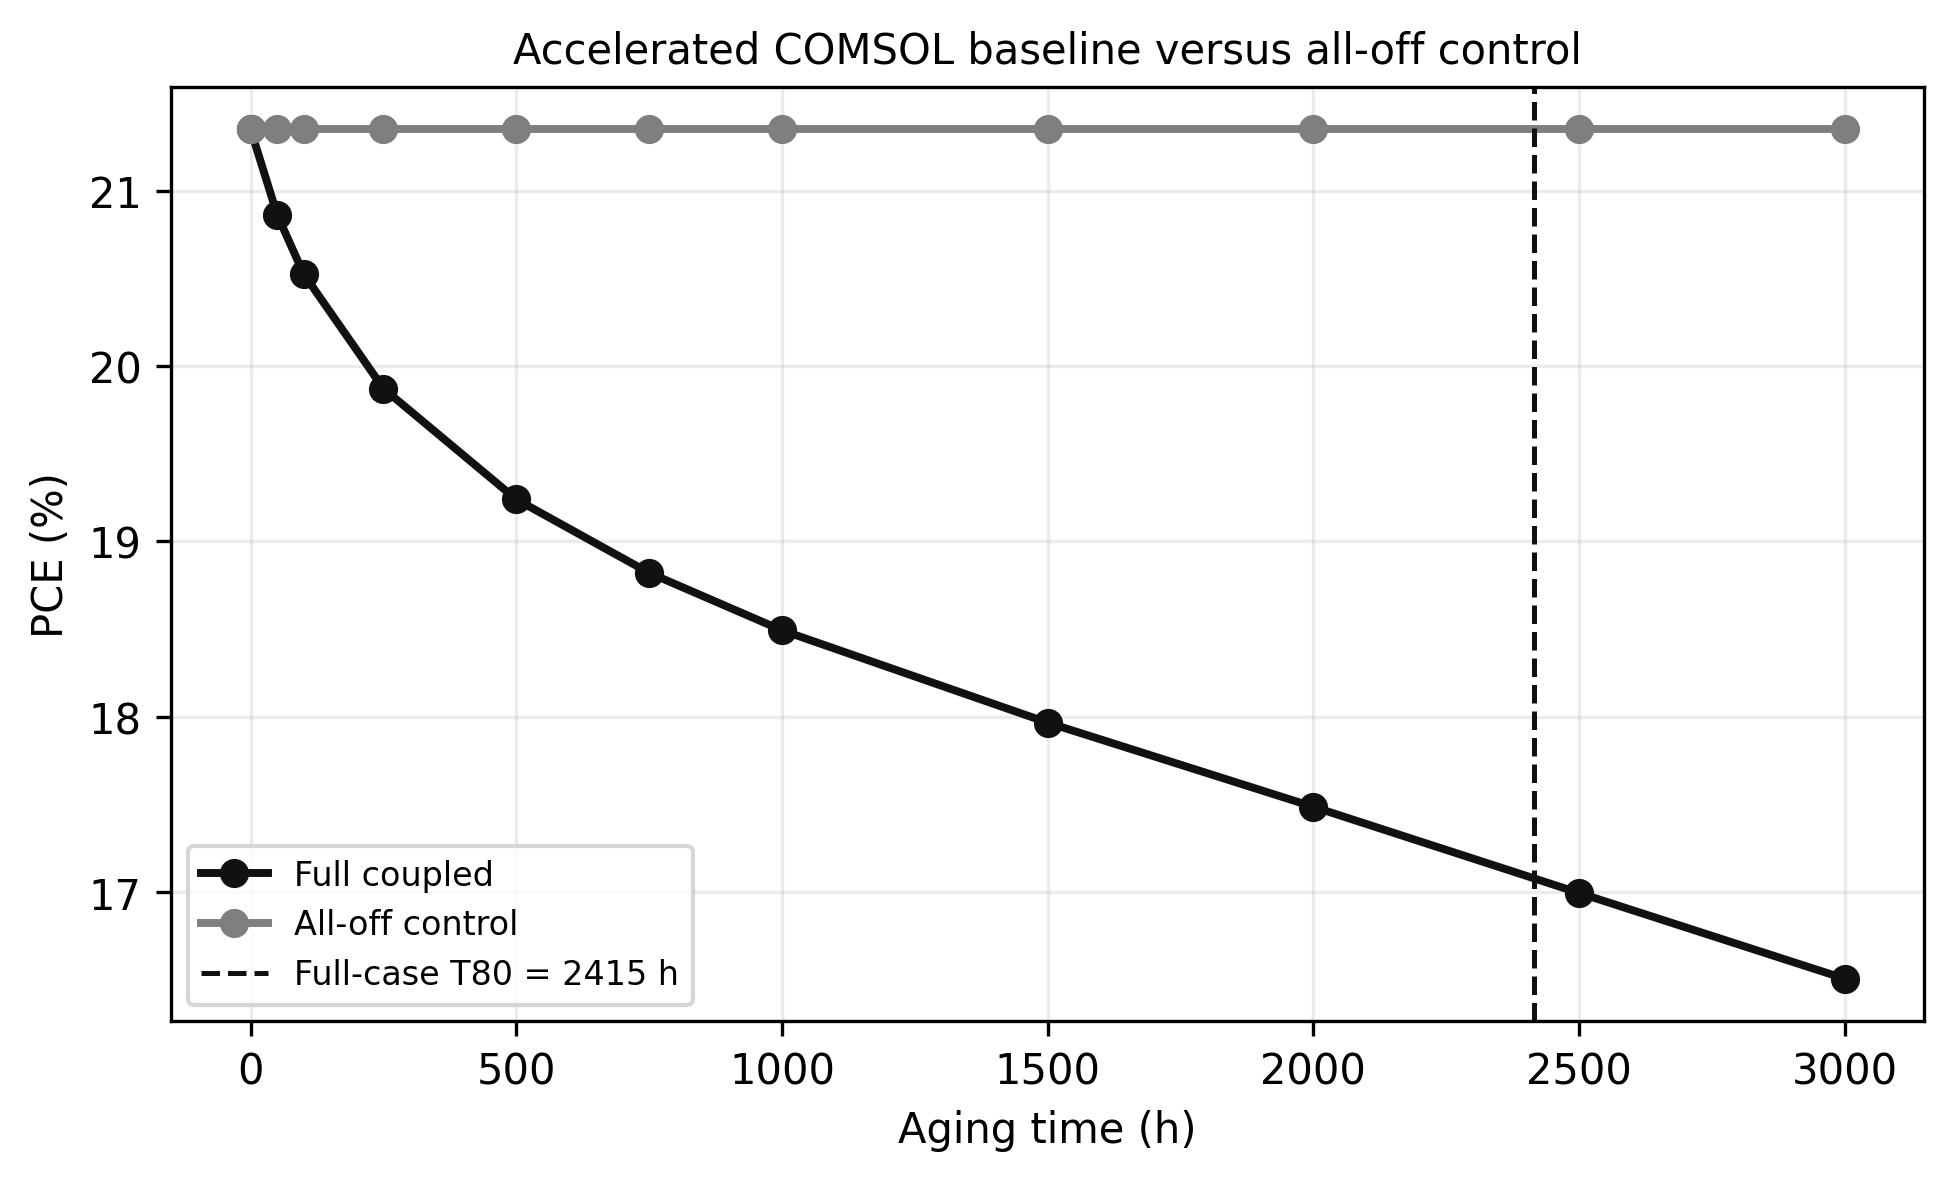
\includegraphics[width=0.82\textwidth]{outputs/figures/comsol_baseline_pce.png}
\caption{COMSOL full coupled degradation baseline compared with the all-off control. The full coupled case reaches interpolated $T_{80}=2415$ h.}
\label{fig:comsol_baseline_pce}
\end{figure}

Figure~\ref{fig:comsol_baseline_pce} shows that the full coupled case loses PCE
while the all-off control remains flat. The variable that changes is the
mechanism-state vector that maps into $N_t$, $R_s$, $R_{sh}$, $Q_f$, and
surface recombination. The equations causing the change are the bounded
degradation mappings described in Chapter~5. Physically, the curve represents
accelerated combined degradation rather than one isolated mechanism. The J--V
signature is a loss in extracted power over aging time. The interpretation is
qualitative until the accelerated degradation amplitudes are calibrated to
matched experimental stress data.

\begin{table}[H]
\centering
\caption{Lifetime summary for the control, full-coupled baseline, and the active one-only and leave-one-out mechanism studies.}
\label{tab:comsol_lifetime_summary}
\small
\begin{tabular}{@{}lrrrrr@{}}
\toprule
scenario & PCE0\_pct & PCE\_3000\_pct & PCE\_retention\_3000 & T90\_h & T80\_h \\
\midrule
full & 21.350 & 16.507 & 0.773 & 515.261 & 2414.671 \\
no Rsh & 21.350 & 18.170 & 0.851 & 601.744 & -- \\
no Nt & 21.350 & 19.698 & 0.923 & -- & -- \\
no Qf & 21.350 & 15.861 & 0.743 & 393.671 & 1768.072 \\
control & 21.350 & 21.350 & 1.000 & -- & -- \\
only Rsh & 21.350 & 19.333 & 0.906 & -- & -- \\
only Nt & 21.350 & 17.444 & 0.817 & 423.679 & -- \\
only Qf & 21.350 & 21.783 & 1.020 & -- & -- \\
\bottomrule
\end{tabular}
\end{table}


Table~\ref{tab:comsol_lifetime_summary} reports the main lifetime markers.
The one-only $N_t$ case produces a large PCE loss but does not cross $T_{80}$
within 3000 h. The one-only $Q_f$ case improves the J--V output in this
parameterization, so removing $Q_f$ from the full coupled case makes
degradation more severe. This counteracting behavior shows why additive
mechanism assumptions should be checked directly in the COMSOL library rather
than assumed to be linear and monotonic.

\section{J--V and State Evolution}

\begin{figure}[H]
\centering
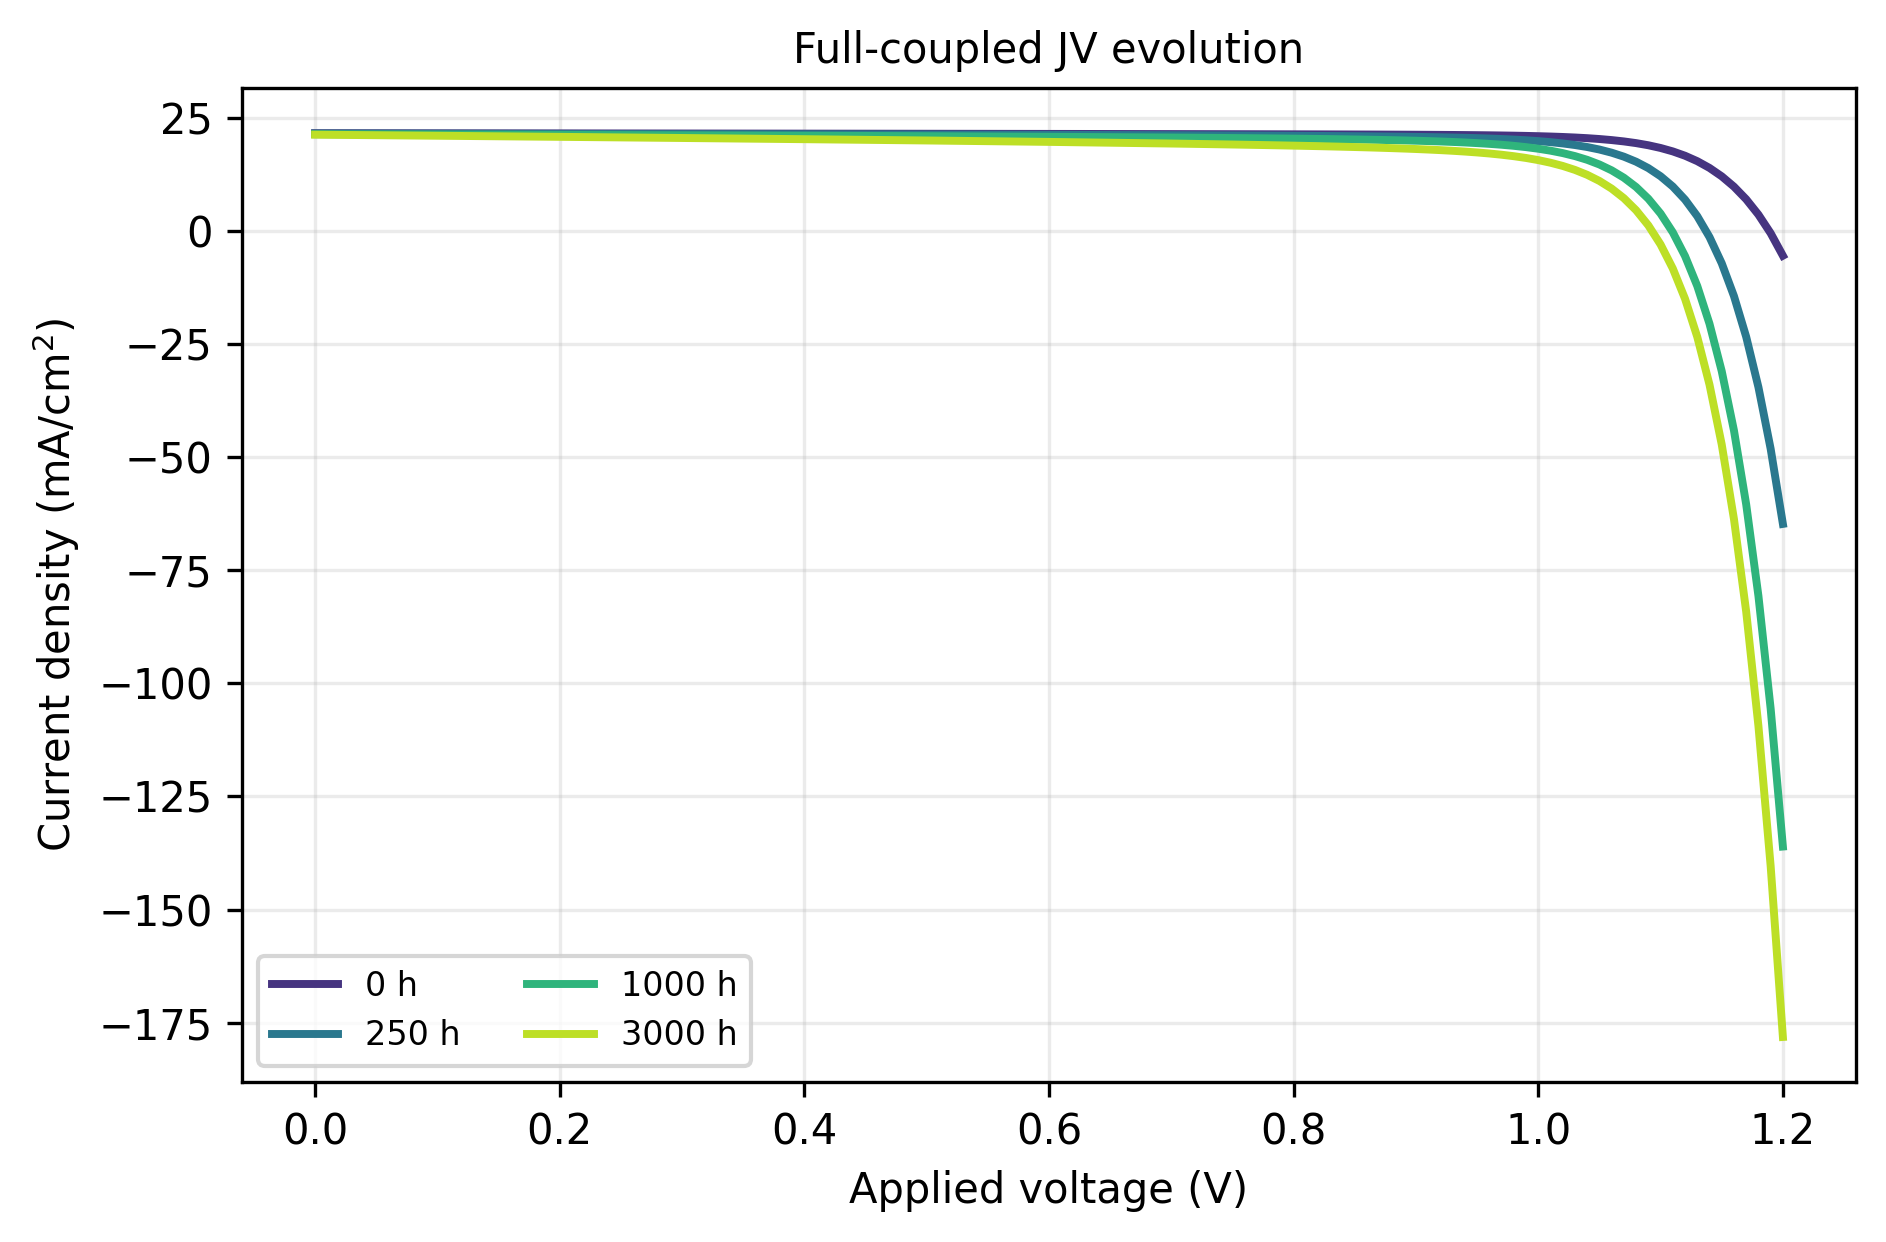
\includegraphics[width=0.82\textwidth]{outputs/figures/comsol_full_jv_evolution.png}
\caption{Full-coupled J--V evolution at selected aging times from the COMSOL sweep.}
\label{fig:comsol_full_jv}
\end{figure}

Figure~\ref{fig:comsol_full_jv} shows the full coupled J--V evolution. The
primary visible change is a downward and leftward shift near the knee region.
The variables that change are the effective recombination and resistance
parameters. Increased $N_t$ increases SRH recombination, reduced $R_{sh}$
increases leakage, and increased $R_s$ adds terminal voltage loss. The physical
mechanisms are trap growth, leakage-path formation, and contact or interface
degradation. The J--V signature is FF loss with accompanying PCE reduction.
The limitation is that similar knee collapse can result from several mechanism
combinations, so the curve shape must be interpreted with state trajectories
and independent calibration data.

\begin{figure}[H]
\centering
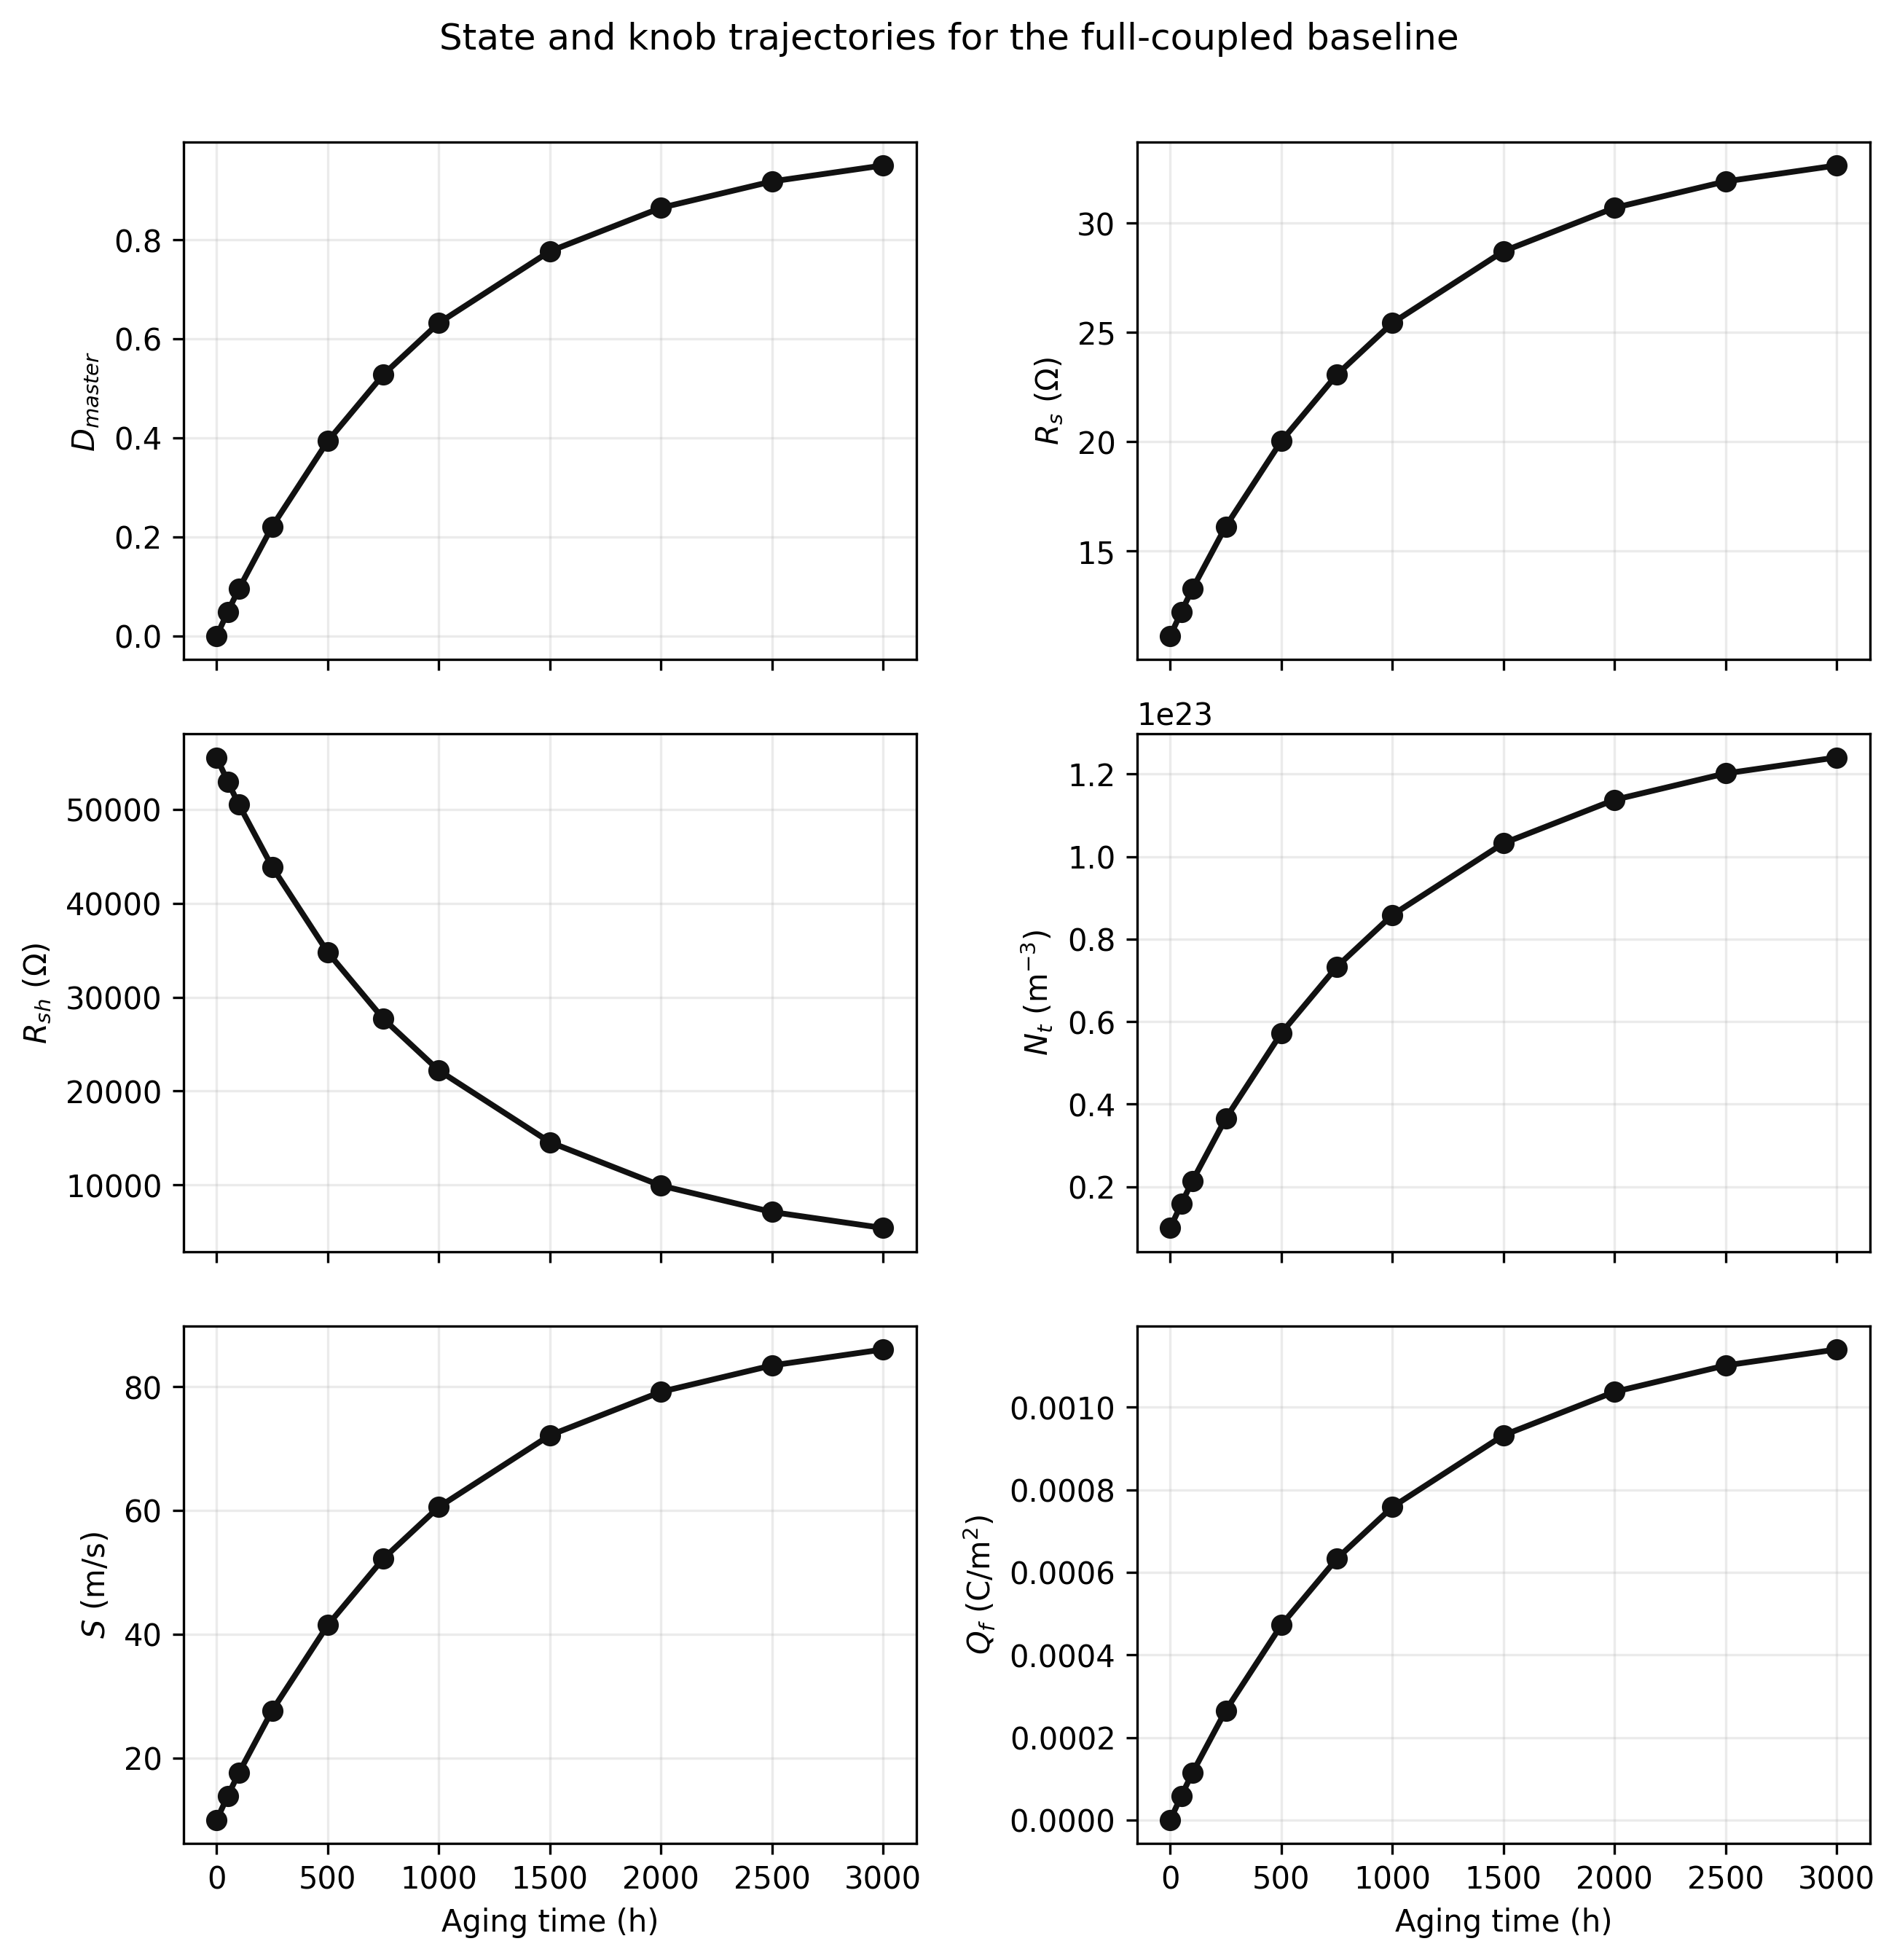
\includegraphics[width=0.92\textwidth]{outputs/figures/comsol_state_trajectories.png}
\caption{State and degradation-knob trajectories for the full coupled COMSOL baseline.}
\label{fig:comsol_state_trajectories}
\end{figure}

Figure~\ref{fig:comsol_state_trajectories} records the corresponding
degradation-parameter trajectories. The figure answers what the electrical
outputs respond to: bounded state variables map into COMSOL parameters over
aging time. This traceability is important because PCE loss alone does not
identify a mechanism. The limitation is that the state trajectories are
simulation inputs or coupled model states, not directly measured material
quantities unless additional experiments are used for calibration.

\section{Mechanism Sensitivity}

\begin{figure}[H]
\centering
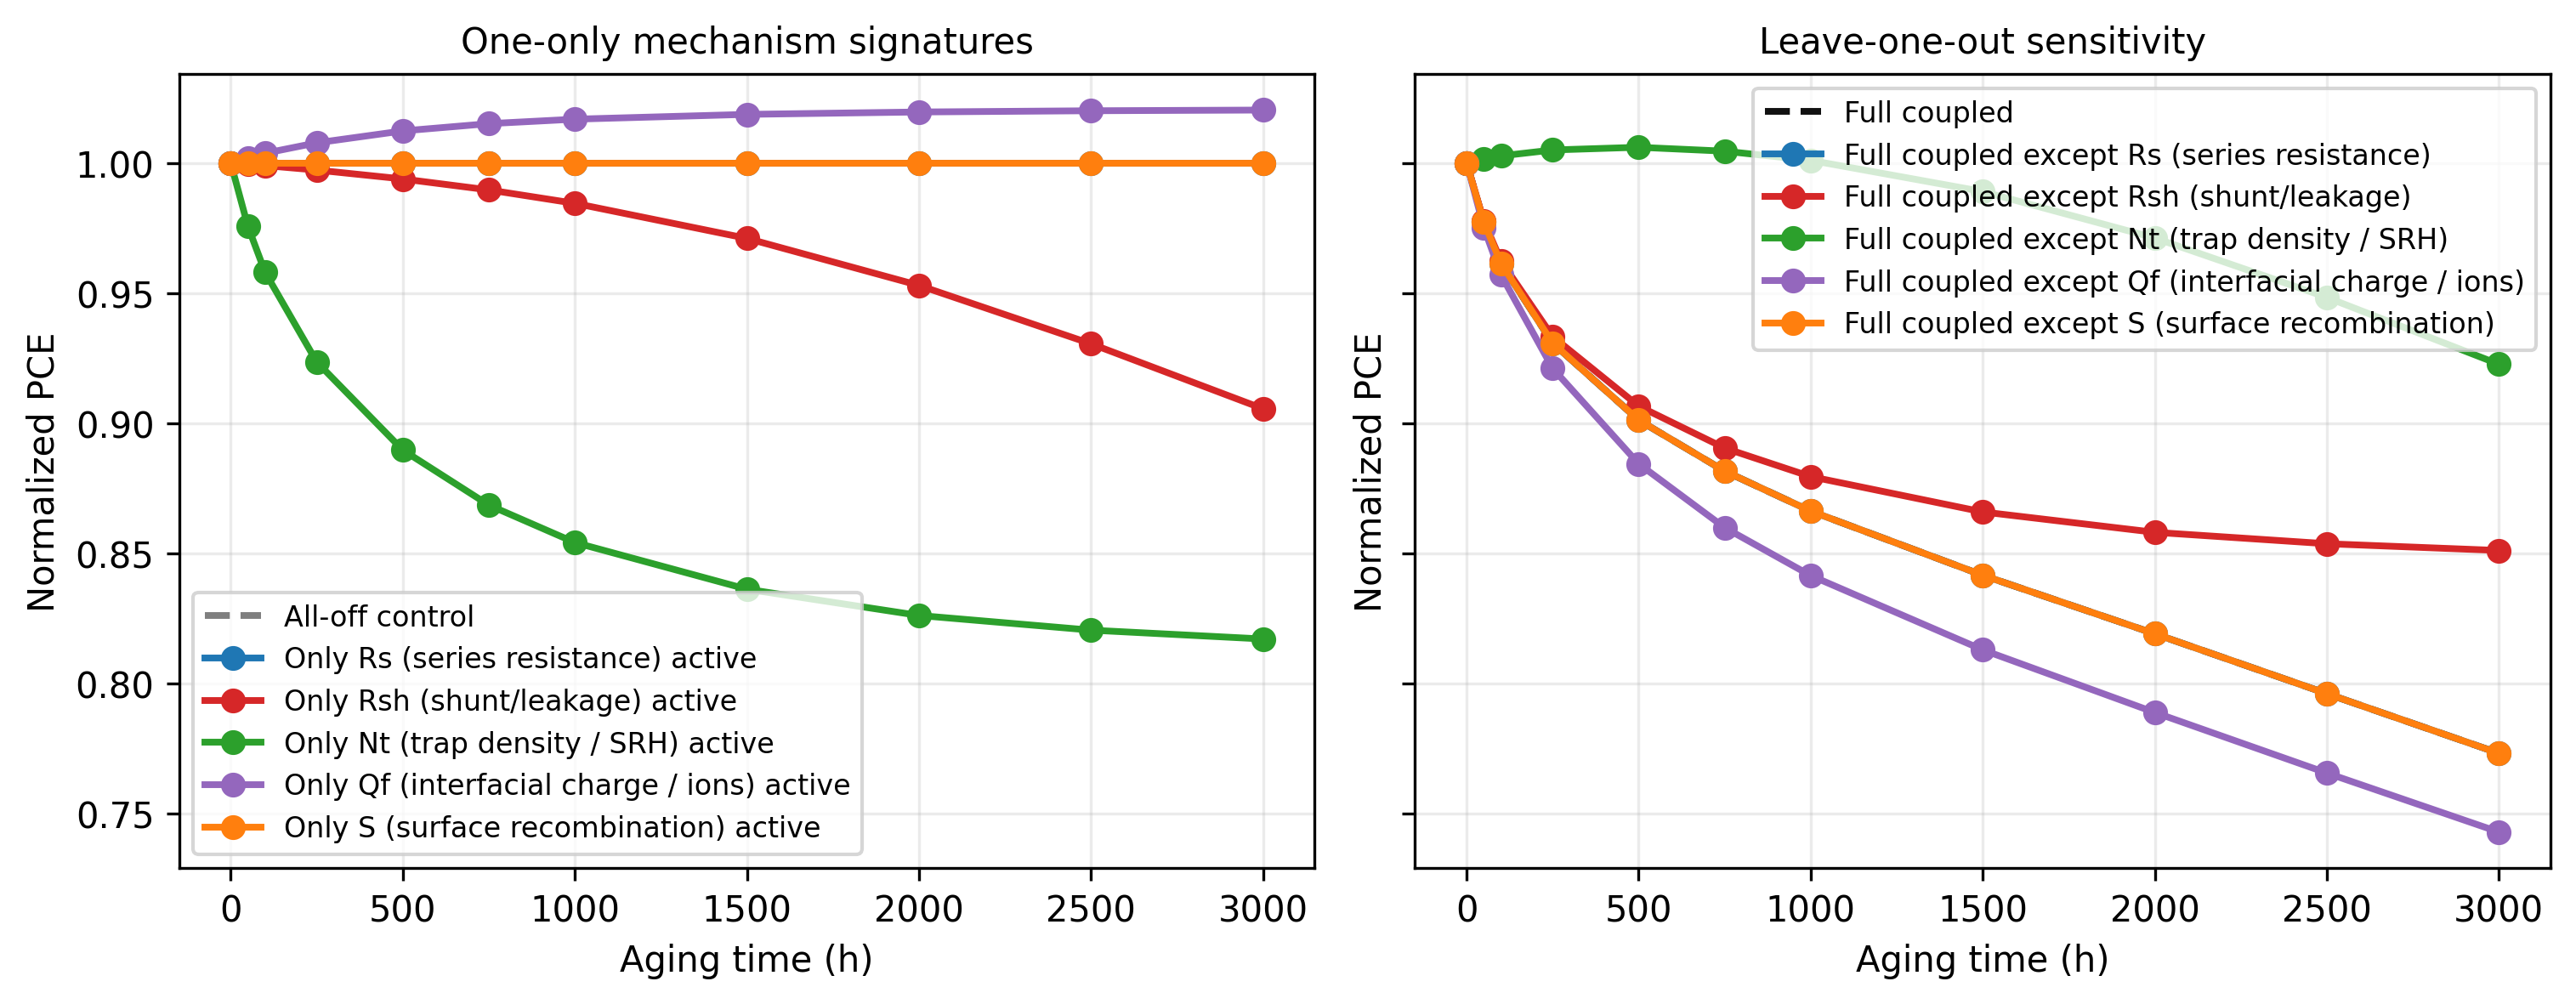
\includegraphics[width=\textwidth]{outputs/figures/comsol_mechanism_sensitivity.png}
\caption{One-only and leave-one-out mechanism sensitivity in the accelerated COMSOL scenario library.}
\label{fig:comsol_mechanism_sensitivity}
\end{figure}

Figure~\ref{fig:comsol_mechanism_sensitivity} compares one-only and
leave-one-out PCE responses. The one-only cases show that $N_t$ and $R_{sh}$
drive the strongest losses among the electrical observables, while $Q_f$ is
counteracting in this parameterization. The governing relations are the trap
density mapping in Eq.~\ref{eq:nt_linear}, the shunt mapping in
Eq.~\ref{eq:rsh_deg}, and the ionic or fixed-charge contribution to Poisson
electrostatics. The physical interpretation is that recombination and leakage
dominate the present terminal metrics, while charge redistribution can either
increase or decrease extracted power depending on how it changes band bending.
The mechanism ranking is qualitative because the amplitudes are selected for mechanism
separation rather than calibrated material degradation.

\begin{figure}[H]
\centering
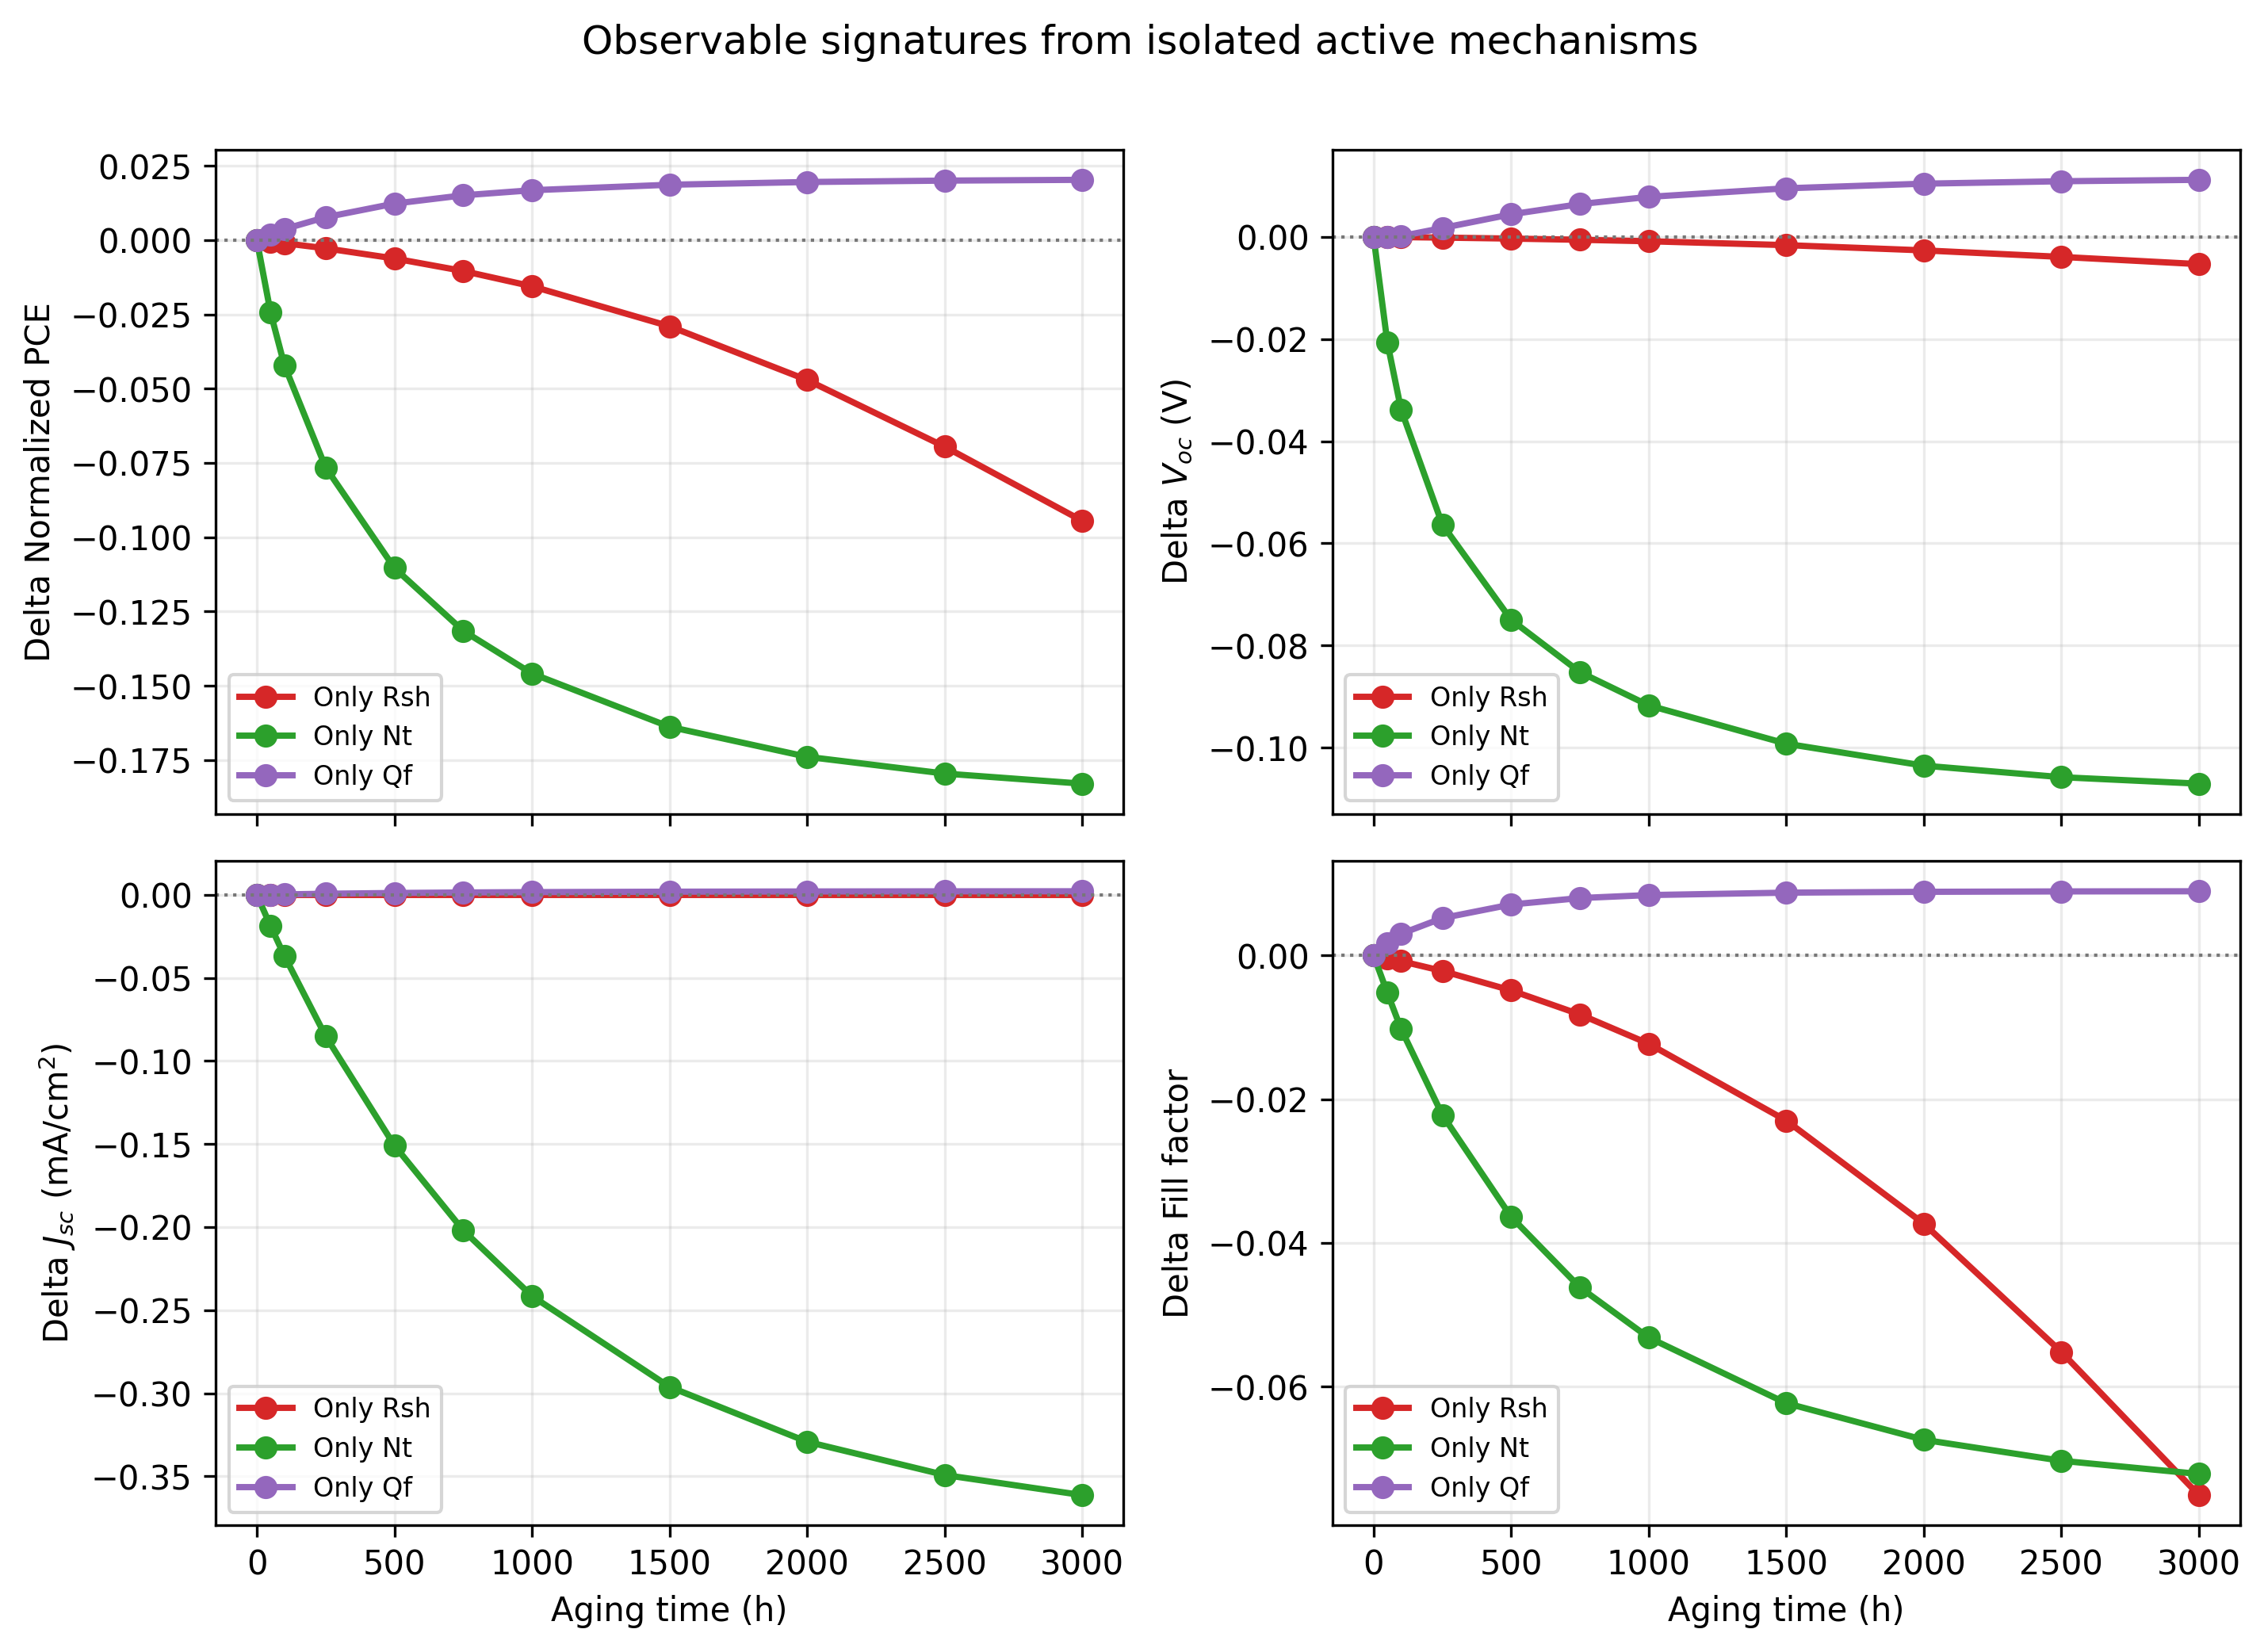
\includegraphics[width=\textwidth]{outputs/figures/comsol_metric_signatures.png}
\caption{Electrical observable signatures from the active one-only COMSOL mechanisms.}
\label{fig:comsol_metric_signatures}
\end{figure}

Figure~\ref{fig:comsol_metric_signatures} separates the J--V-derived metrics.
The $N_t$ case changes $V_{oc}$, $J_{sc}$, FF, and PCE because lifetime
reduction affects both voltage and collection. The $R_{sh}$ case is more
fill-factor dominated because leakage changes the low-bias slope. The $Q_f$
case has a smaller but nonzero counteracting signature because electrostatic
charge modifies internal fields. These signatures are useful for calibration
planning, but terminal metrics alone cannot uniquely identify all mechanisms.

\section{Electronic Parameter Sweep}

A separate COMSOL Global Evaluation export was used to sweep the baseline
electronic parameters $N_{t,0}$, $R_{s,0}$, and $R_{sh,0}$. Unlike the aging
library above, this sweep is not a time-evolving degradation trajectory. It is a
local electronic sensitivity study that checks whether the terminal J--V
signatures respond to the expected physical parameter directions. The export
contains 819 parameter combinations. The post-processing script extracts the
active voltage-ramp segment from each transient scan and computes PCE,
$V_{oc}$, $J_{sc}$, FF, $V_{\mathrm{mpp}}$, and $J_{\mathrm{mpp}}$.

\begin{table}[H]
\centering
\caption{Summary of the one-parameter-at-a-time COMSOL electronic sweep. The
held parameters are fixed at the model reference values:
$N_{t,0}=10^{16}~\mathrm{cm^{-3}}$, $R_{s,0}=1~\Omega\mathrm{cm^2}$, and
$R_{sh,0}=10^{5}~\Omega\mathrm{cm^2}$. The PCE ranges report the extrema from
that one-parameter-at-a-time slice, not the best point from the full
all-combination grid.}
\label{tab:parameter_sweep_summary}
\begin{tabular}{@{}p{0.13\textwidth}p{0.25\textwidth}p{0.17\textwidth}p{0.34\textwidth}@{}}
\toprule
Sweep & Parameter range & PCE range & Main response and interpretation \\
\midrule
$N_{t,0}$ &
$10^{14}$--$10^{20}~\mathrm{cm^{-3}}$ &
19.01--17.08\% &
$V_{oc}$ and $J_{sc}$ decrease, consistent with stronger bulk recombination. \\
$R_{s,0}$ &
0.1--$10~\Omega\mathrm{cm^2}$ &
19.42--15.90\% &
FF decreases from 0.812 to 0.665, consistent with series loss. \\
$R_{sh,0}$ &
$10^{3}$--$10^{6}~\Omega\mathrm{cm^2}$ &
18.06--19.01\% &
FF improves from 0.757 to 0.795 as leakage is suppressed. \\
\bottomrule
\end{tabular}
\end{table}

\begin{figure}[H]
\centering
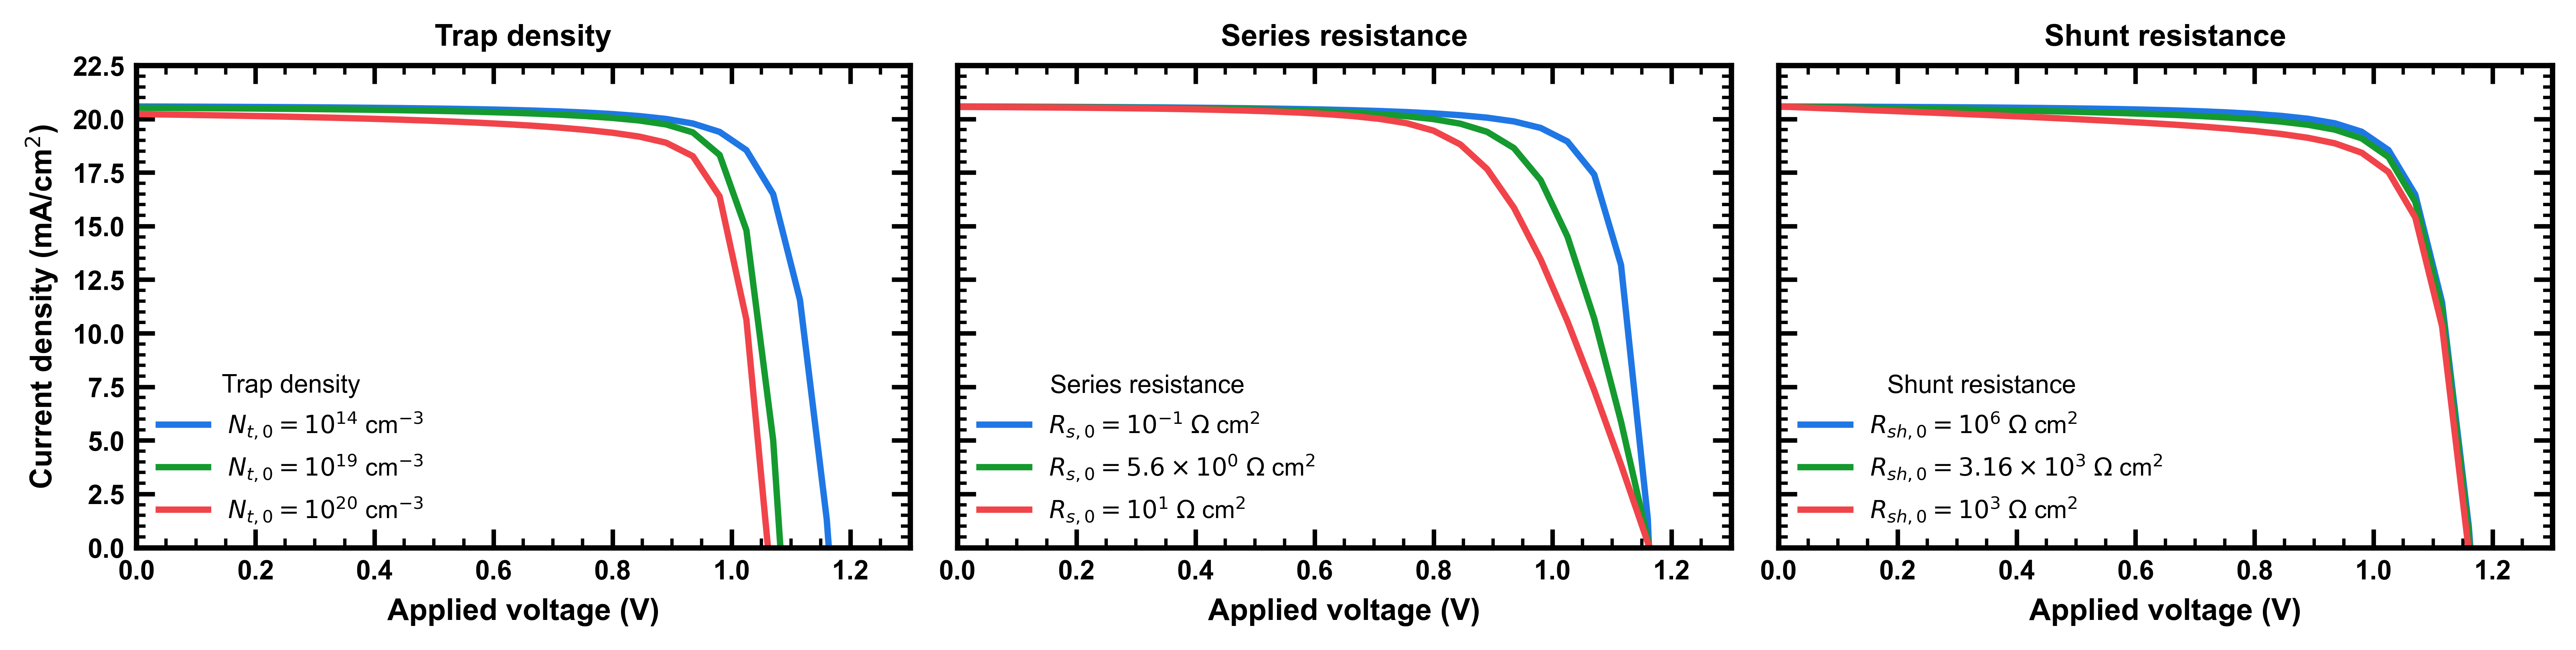
\includegraphics[width=\textwidth]{outputs/figures/comsol_parameter_sweep/comsol_parameter_sweep_jv_examples.png}
\caption{Representative J--V curves from the COMSOL electronic parameter
sweep. Each panel varies one parameter while holding the other two at the
baseline values used in Table~\ref{tab:parameter_sweep_summary}.}
\label{fig:comsol_parameter_sweep_jv}
\end{figure}

Figure~\ref{fig:comsol_parameter_sweep_jv} shows the expected qualitative
terminal signatures. Larger $R_{s,0}$ reduces the high-power knee and lowers
fill factor. Lower $R_{sh,0}$ increases leakage and reduces the low-bias
quality of the curve. Larger $N_{t,0}$ reduces the achievable voltage and
current through recombination. These trends support the interpretation of the
mechanism-isolation library, but they still do not uniquely invert a measured
J--V curve to one material parameter.

\begin{figure}[H]
\centering
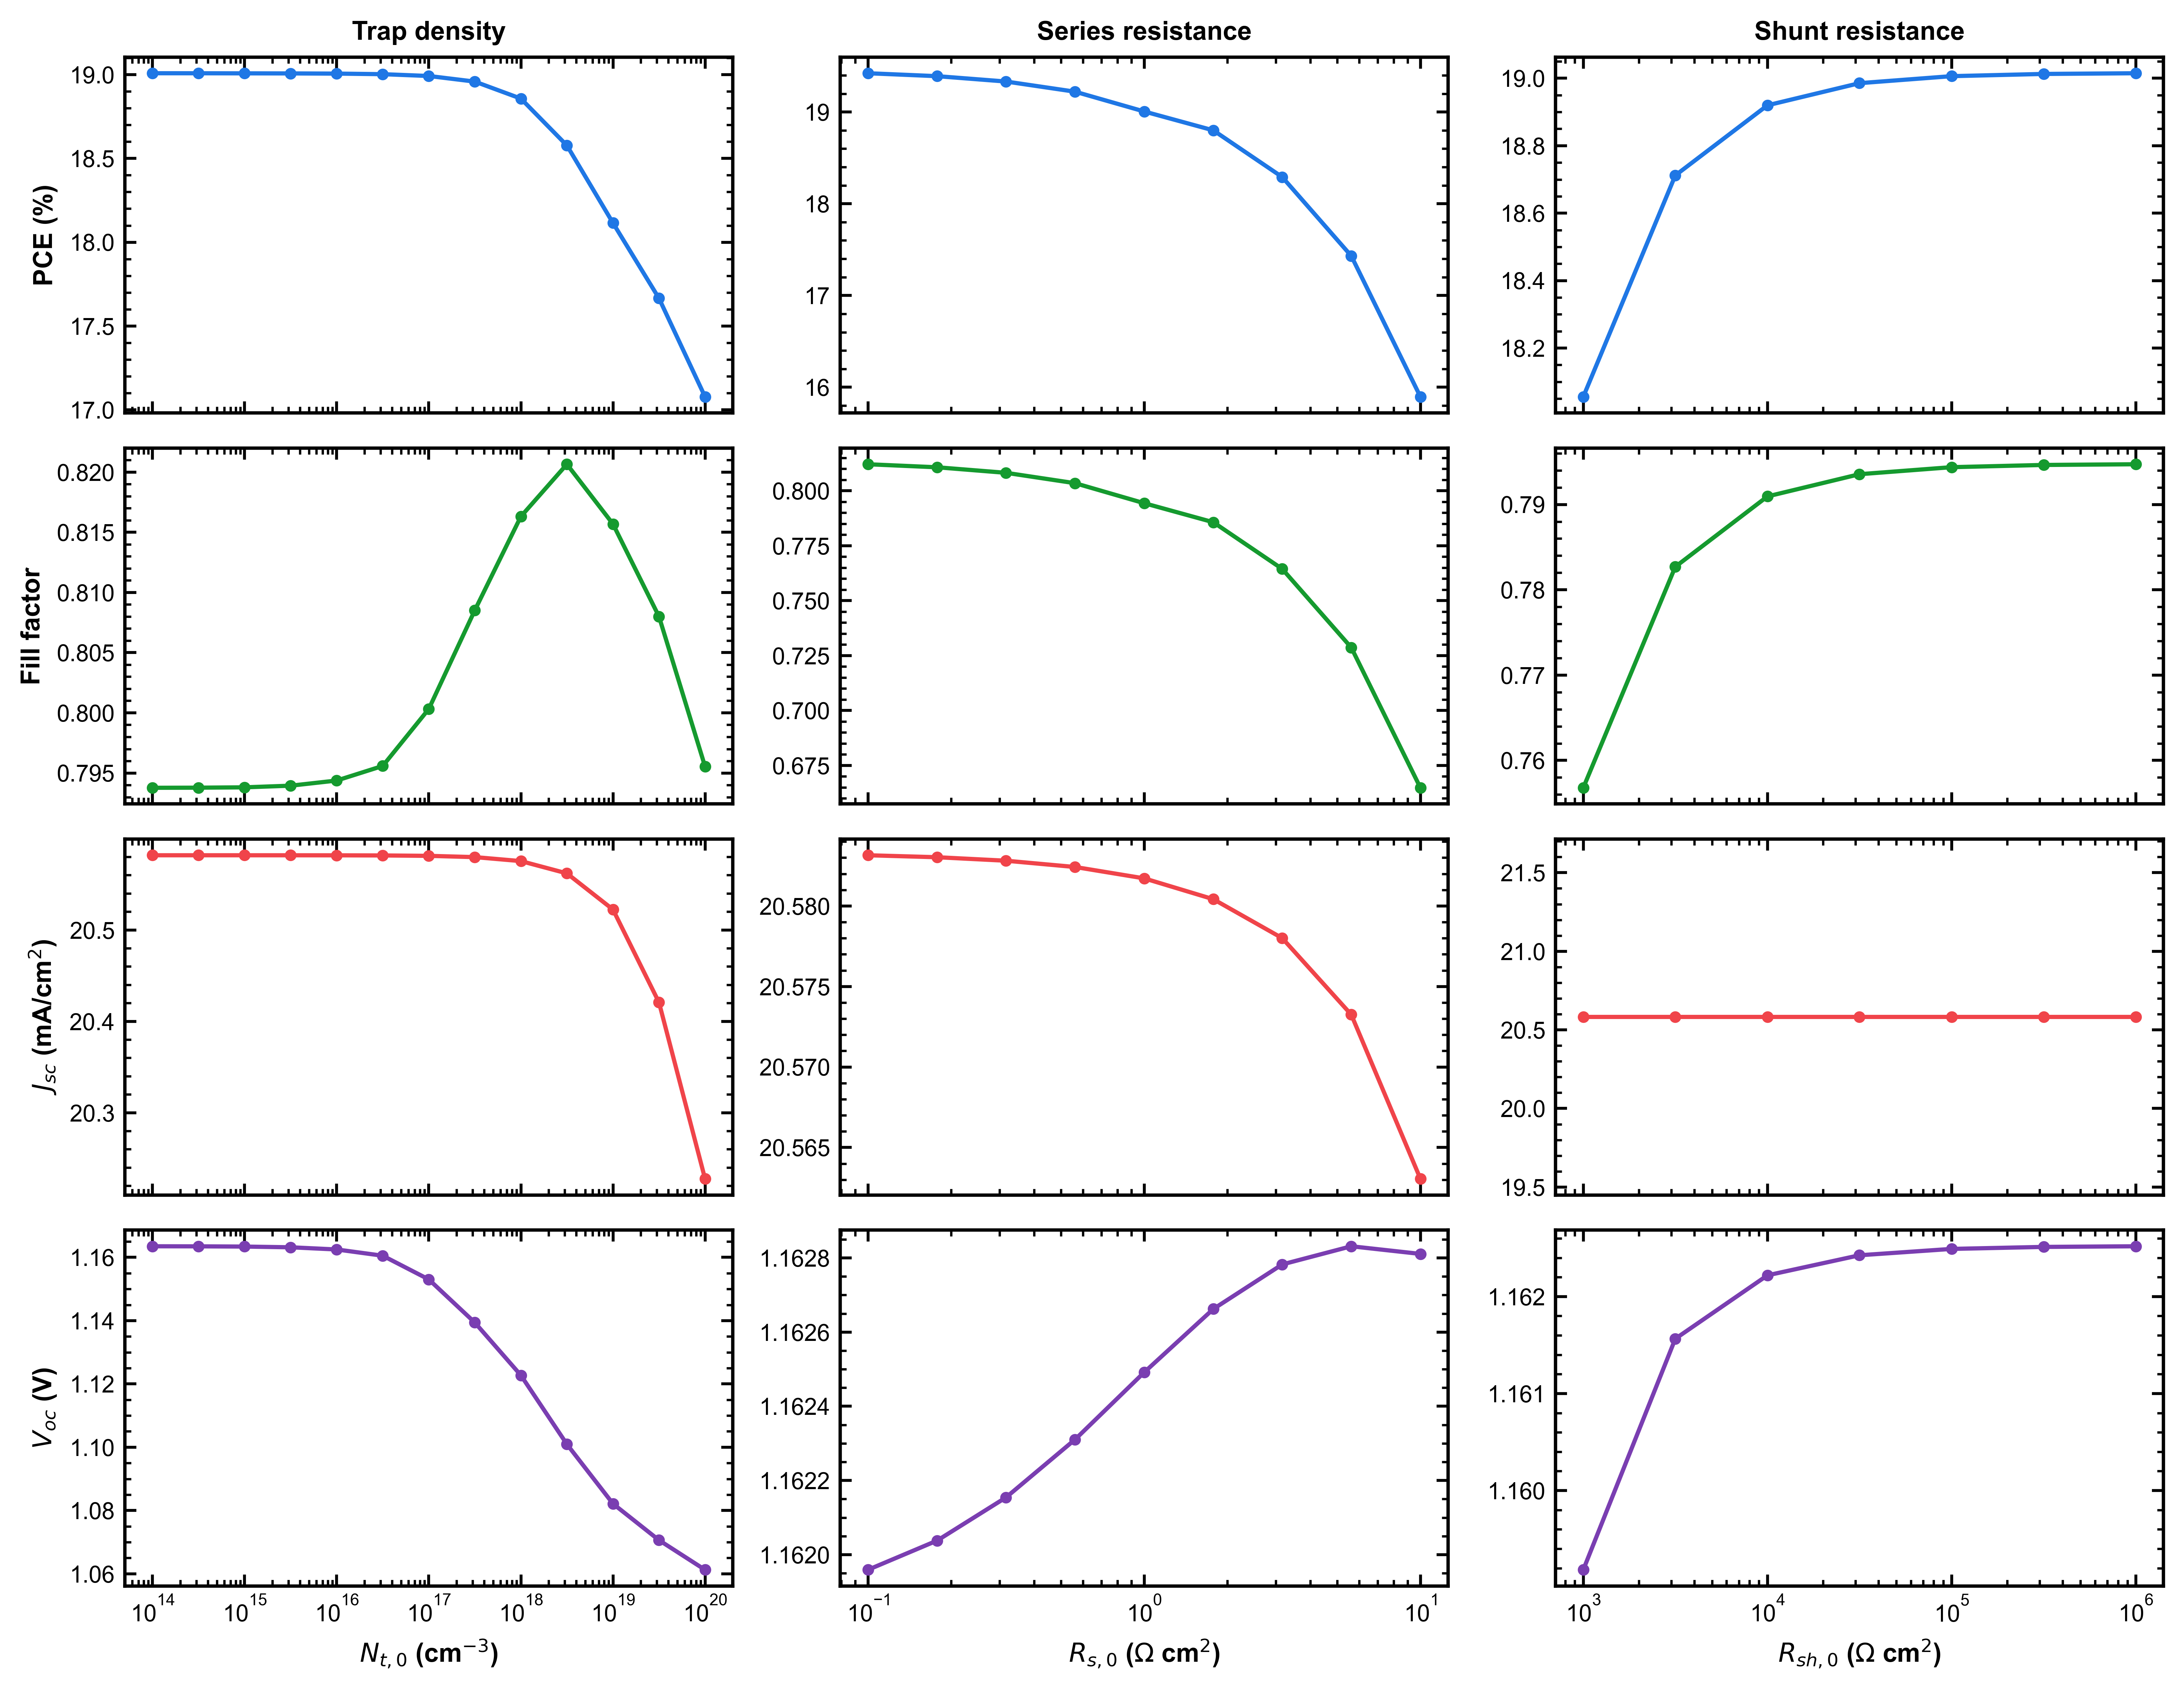
\includegraphics[width=\textwidth]{outputs/figures/comsol_parameter_sweep/comsol_parameter_sweep_metrics_all.png}
\caption{Extracted PCE, fill factor, $J_{sc}$, and $V_{oc}$ for the
one-parameter-at-a-time COMSOL electronic sweep. The full processed table
contains 819 all-combination rows, of which 795 remain above 15\% PCE in this
export.}
\label{fig:comsol_parameter_sweep_metrics}
\end{figure}

Figure~\ref{fig:comsol_parameter_sweep_metrics} converts the J--V curves into
scalar photovoltaic metrics. In this export, the best-performing full-factorial
grid point
has PCE $=19.44\%$, $V_{oc}=1.163$ V, $J_{sc}=20.58~\mathrm{mA/cm^2}$, and
FF $=0.812$. The all-combination sweep spans 13.42--19.44\% PCE. This range is
useful for identifying plausible calibration directions and for defining
future surrogate-model input ranges. It should not be interpreted as an
optimized device design because optical, transport-layer, ion, and degradation
parameters remain fixed.

\section{Architecture-Stress Aging Grid}

The later COMSOL exports extend the thesis data set from static electronic
parameter sweeps to architecture-scoped aging outputs. The current canonical
architecture-stress J--V export,
\path{data/raw/comsol/arch_baseline_pin/Aging/Stress_matrix_jv_003.csv},
stores a full light-temperature diagnostic J--V sweep as a concatenated
two-column table. The post-processing script splits this file into 360 J--V
curves using the COMSOL parameter ordering shown in the export: ten aging
checkpoints and 36 light-temperature scenarios. The scenario grid matches the
profile-grid stress matrix, with aging temperatures of 300--400 K and aging
displayed light levels of 0--1.00 sun, where the plotted 0-sun case is the
COMSOL 0.01-sun numerical floor. This export gives a direct electrical map of
the light-plus-temperature degradation surface. The voltage range ends at
1.25 V, so some low-temperature and early-aging curves do not cross zero
current. PCE and $J_{sc}$ are therefore retained for all curves, while
$V_{oc}$ and FF are reported only for curves with a resolved zero-current
crossing. Earlier files in the same folder,
\path{Stress_matrix_jv_001.csv} and \path{Stress_matrix_jv_002.csv}, are
superseded development exports and are retained only for audit history.

\begin{figure}[H]
\centering
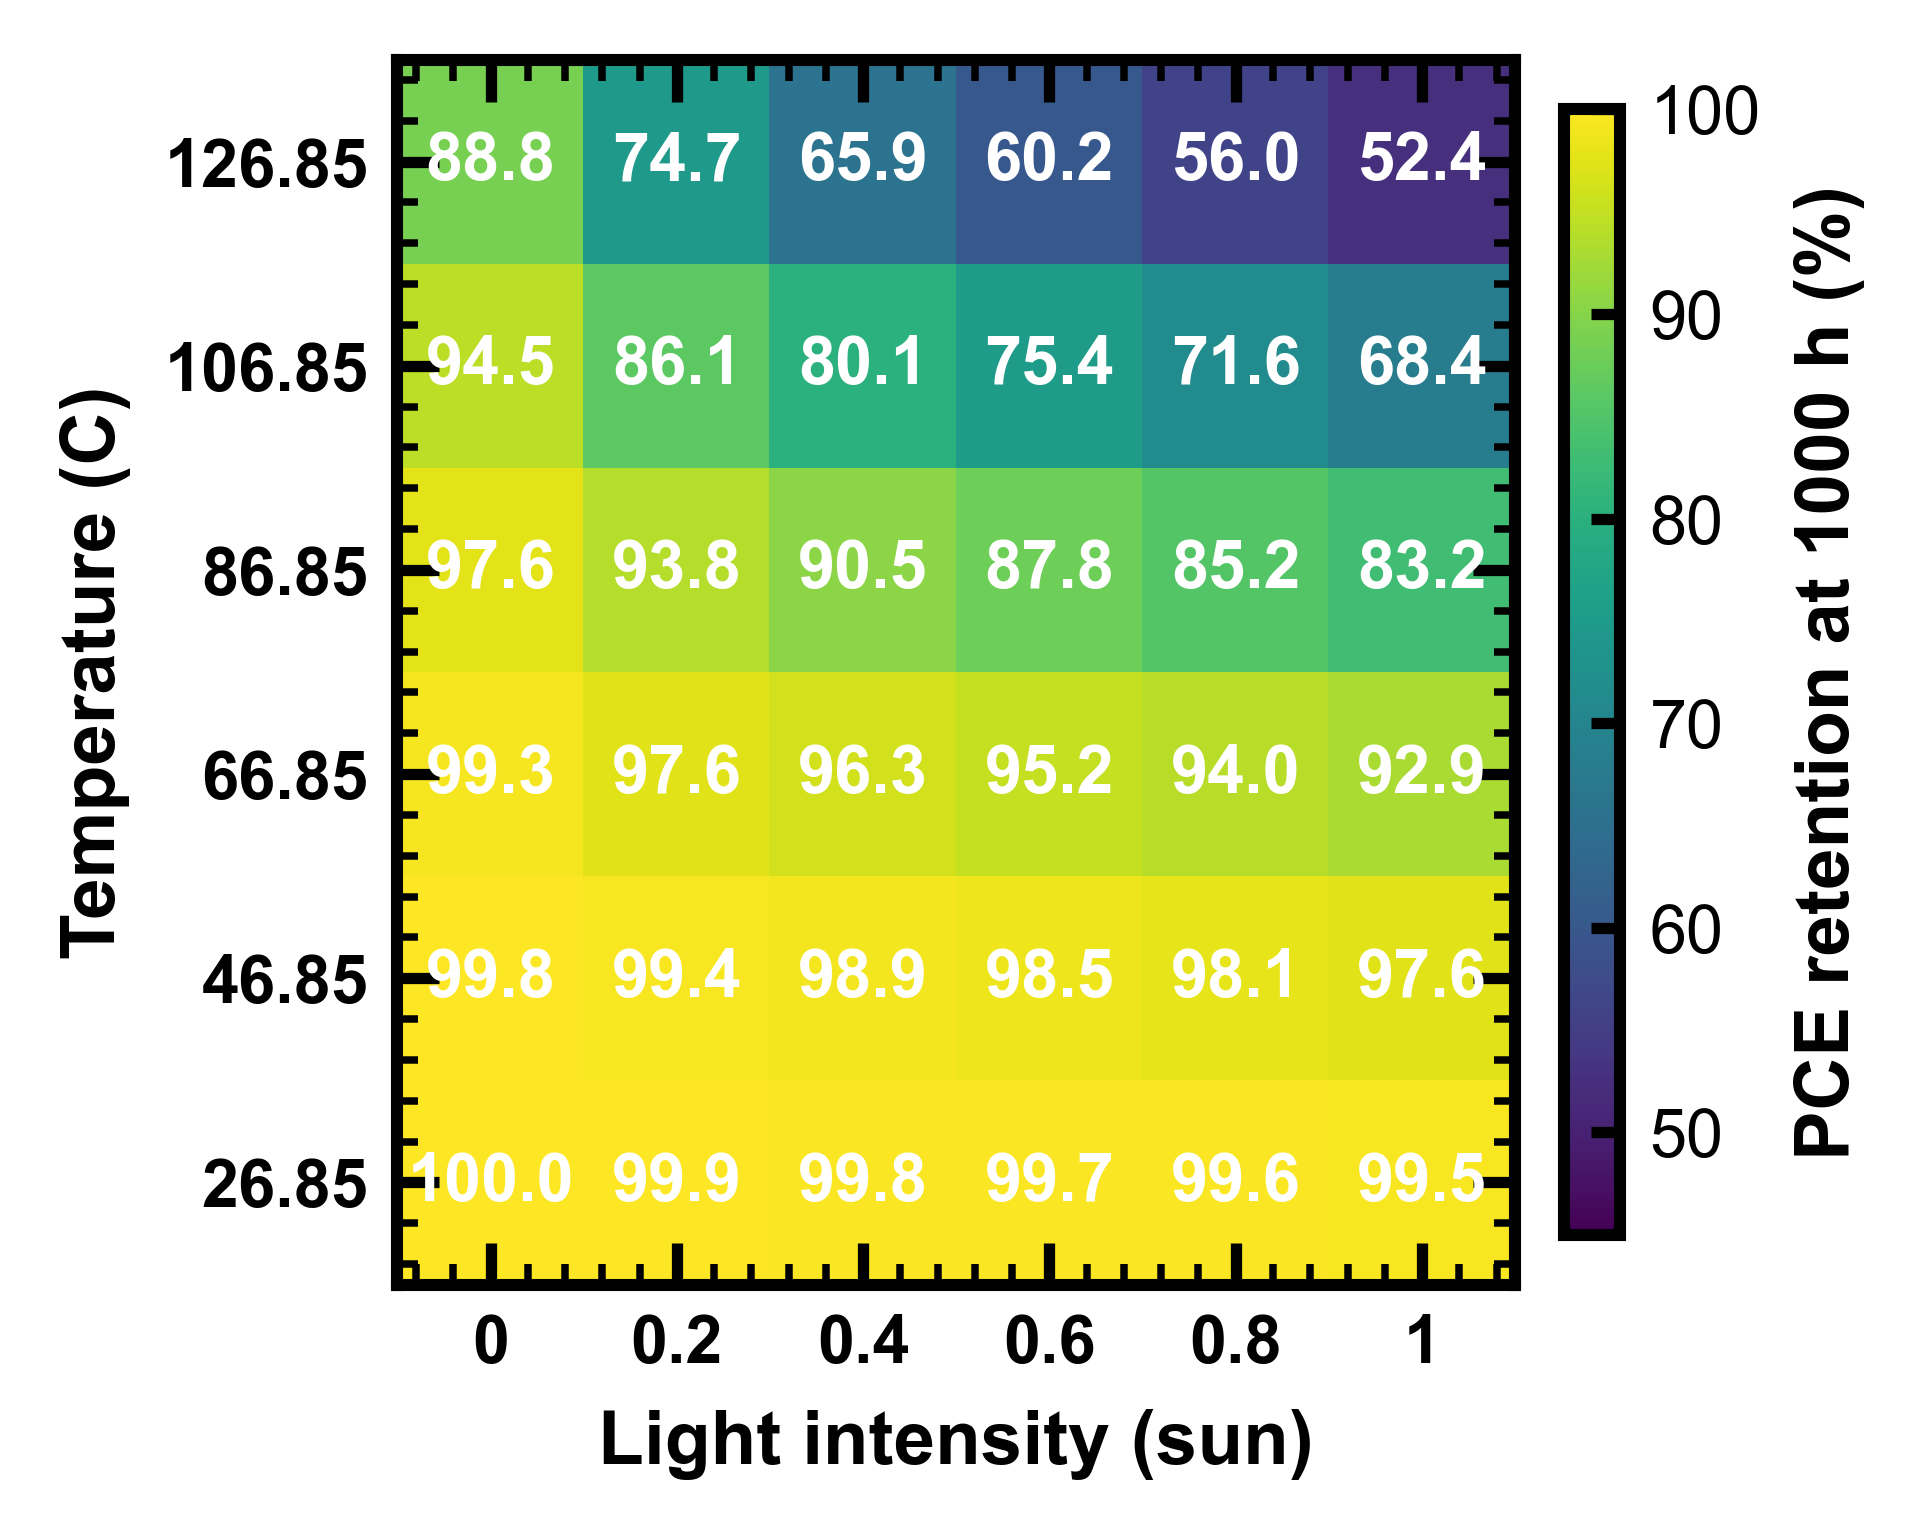
\includegraphics[width=0.72\textwidth]{outputs/figures/comsol_architecture_stress_grid/baseline_pin_stress_matrix_jv_003_pce_retention_heatmap.png}
\caption{Final PCE retention from the 360-curve light-temperature J--V export. The result shows coupled light and heat acceleration: 1000 h retention remains near 100\% at 300 K and low light, but decreases to 52.4\% at 400 K and one sun.}
\label{fig:baseline_pin_temperature_pce_retention_flat}
\end{figure}

\begin{figure}[H]
\centering
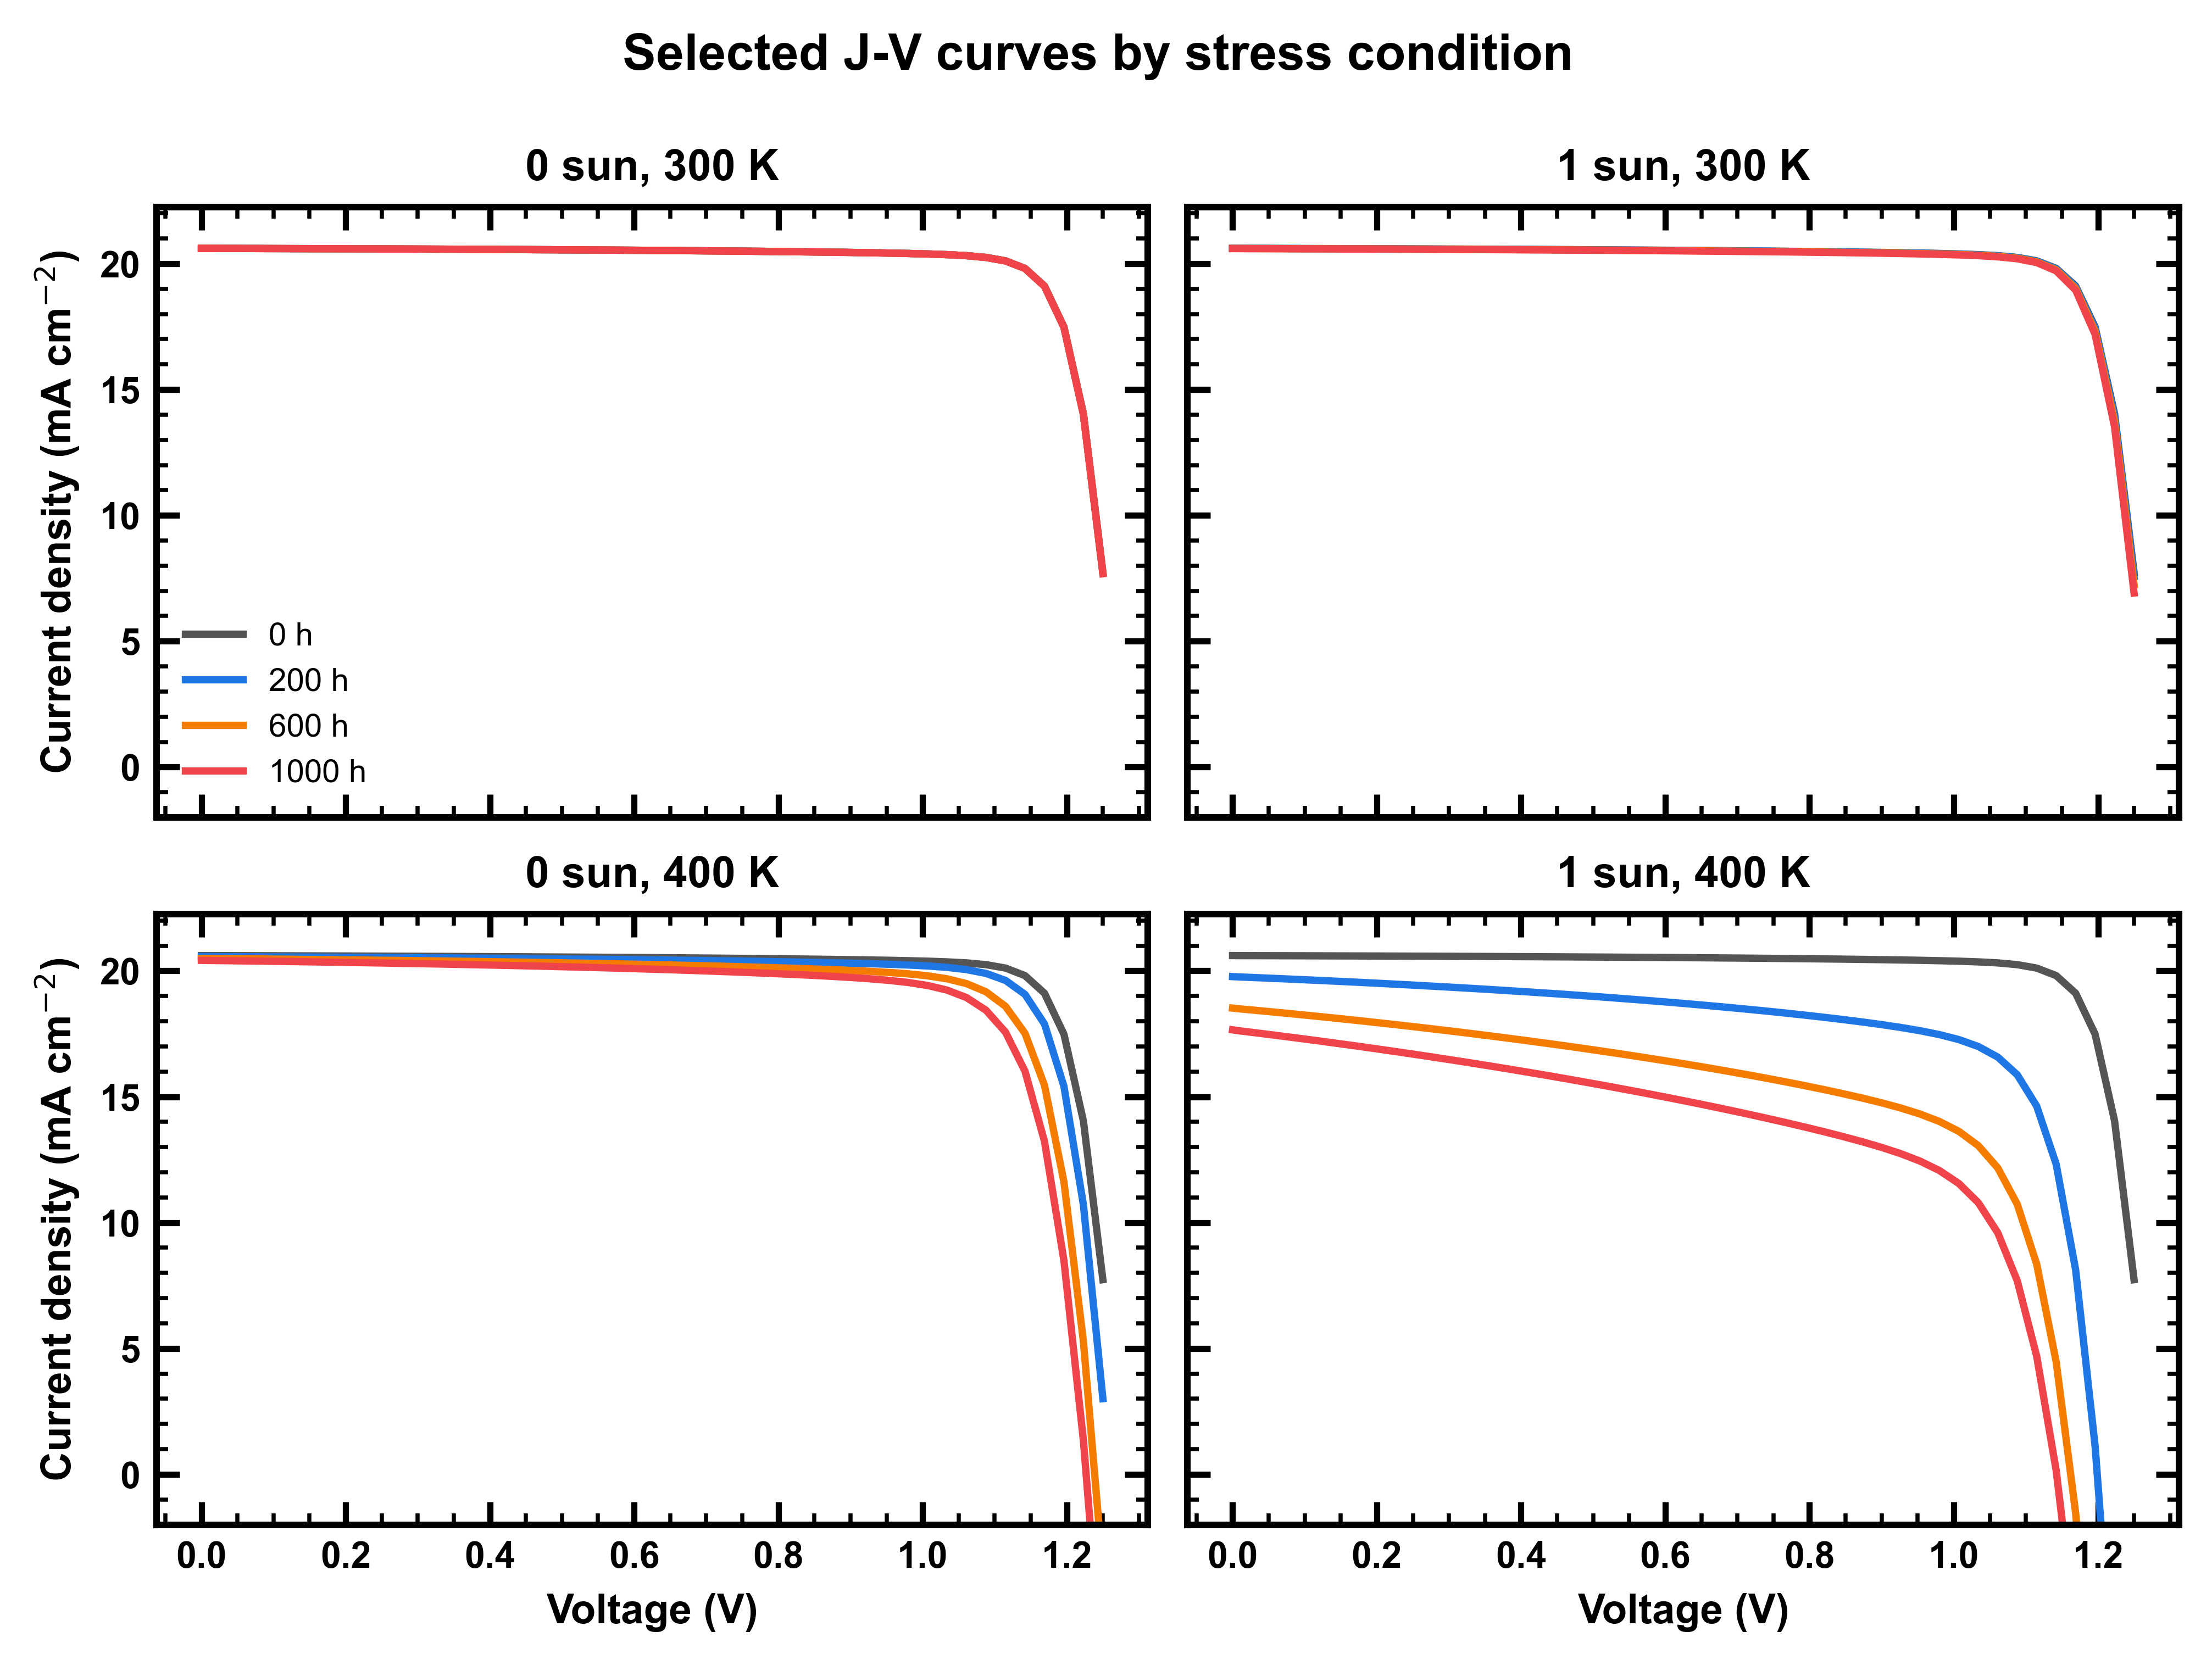
\includegraphics[width=\textwidth]{outputs/figures/comsol_architecture_stress_grid/baseline_pin_stress_matrix_jv_003_jv_selected.png}
\caption{Representative corner J--V curves from the flat light-temperature export. The high-temperature, one-sun case shows stronger $J_{sc}$ loss and knee rounding with aging, while the low-temperature cases remain close to the initial curve over the same equivalent aging window.}
\label{fig:baseline_pin_temperature_jv_flat}
\end{figure}

\section{Light-Temperature Internal-State Profile Grid}

A separate 6 $\times$ 6 profile-grid export was organized for the baseline
p-i-n architecture. It covers aging temperatures of 300, 320, 340, 360, 380,
and 400 K and displayed aging light levels of 0, 0.20, 0.40, 0.60, 0.80, and
1.00 sun. The 0-sun label corresponds to the COMSOL 0.01-sun numerical floor.
Each file contains spatial profiles at ten aging checkpoints for
$u_{\mathrm{ion}}$, $D_{\mathrm{trap}}$, $D_{Rs}$, $D_{Rsh}$,
$N_{t,\mathrm{eff}}$, SRH recombination, and electric field. This grid is the
first data product in the thesis that directly connects terminal J--V trends
to internal state variables across a light-temperature stress matrix.

\begin{figure}[H]
\centering
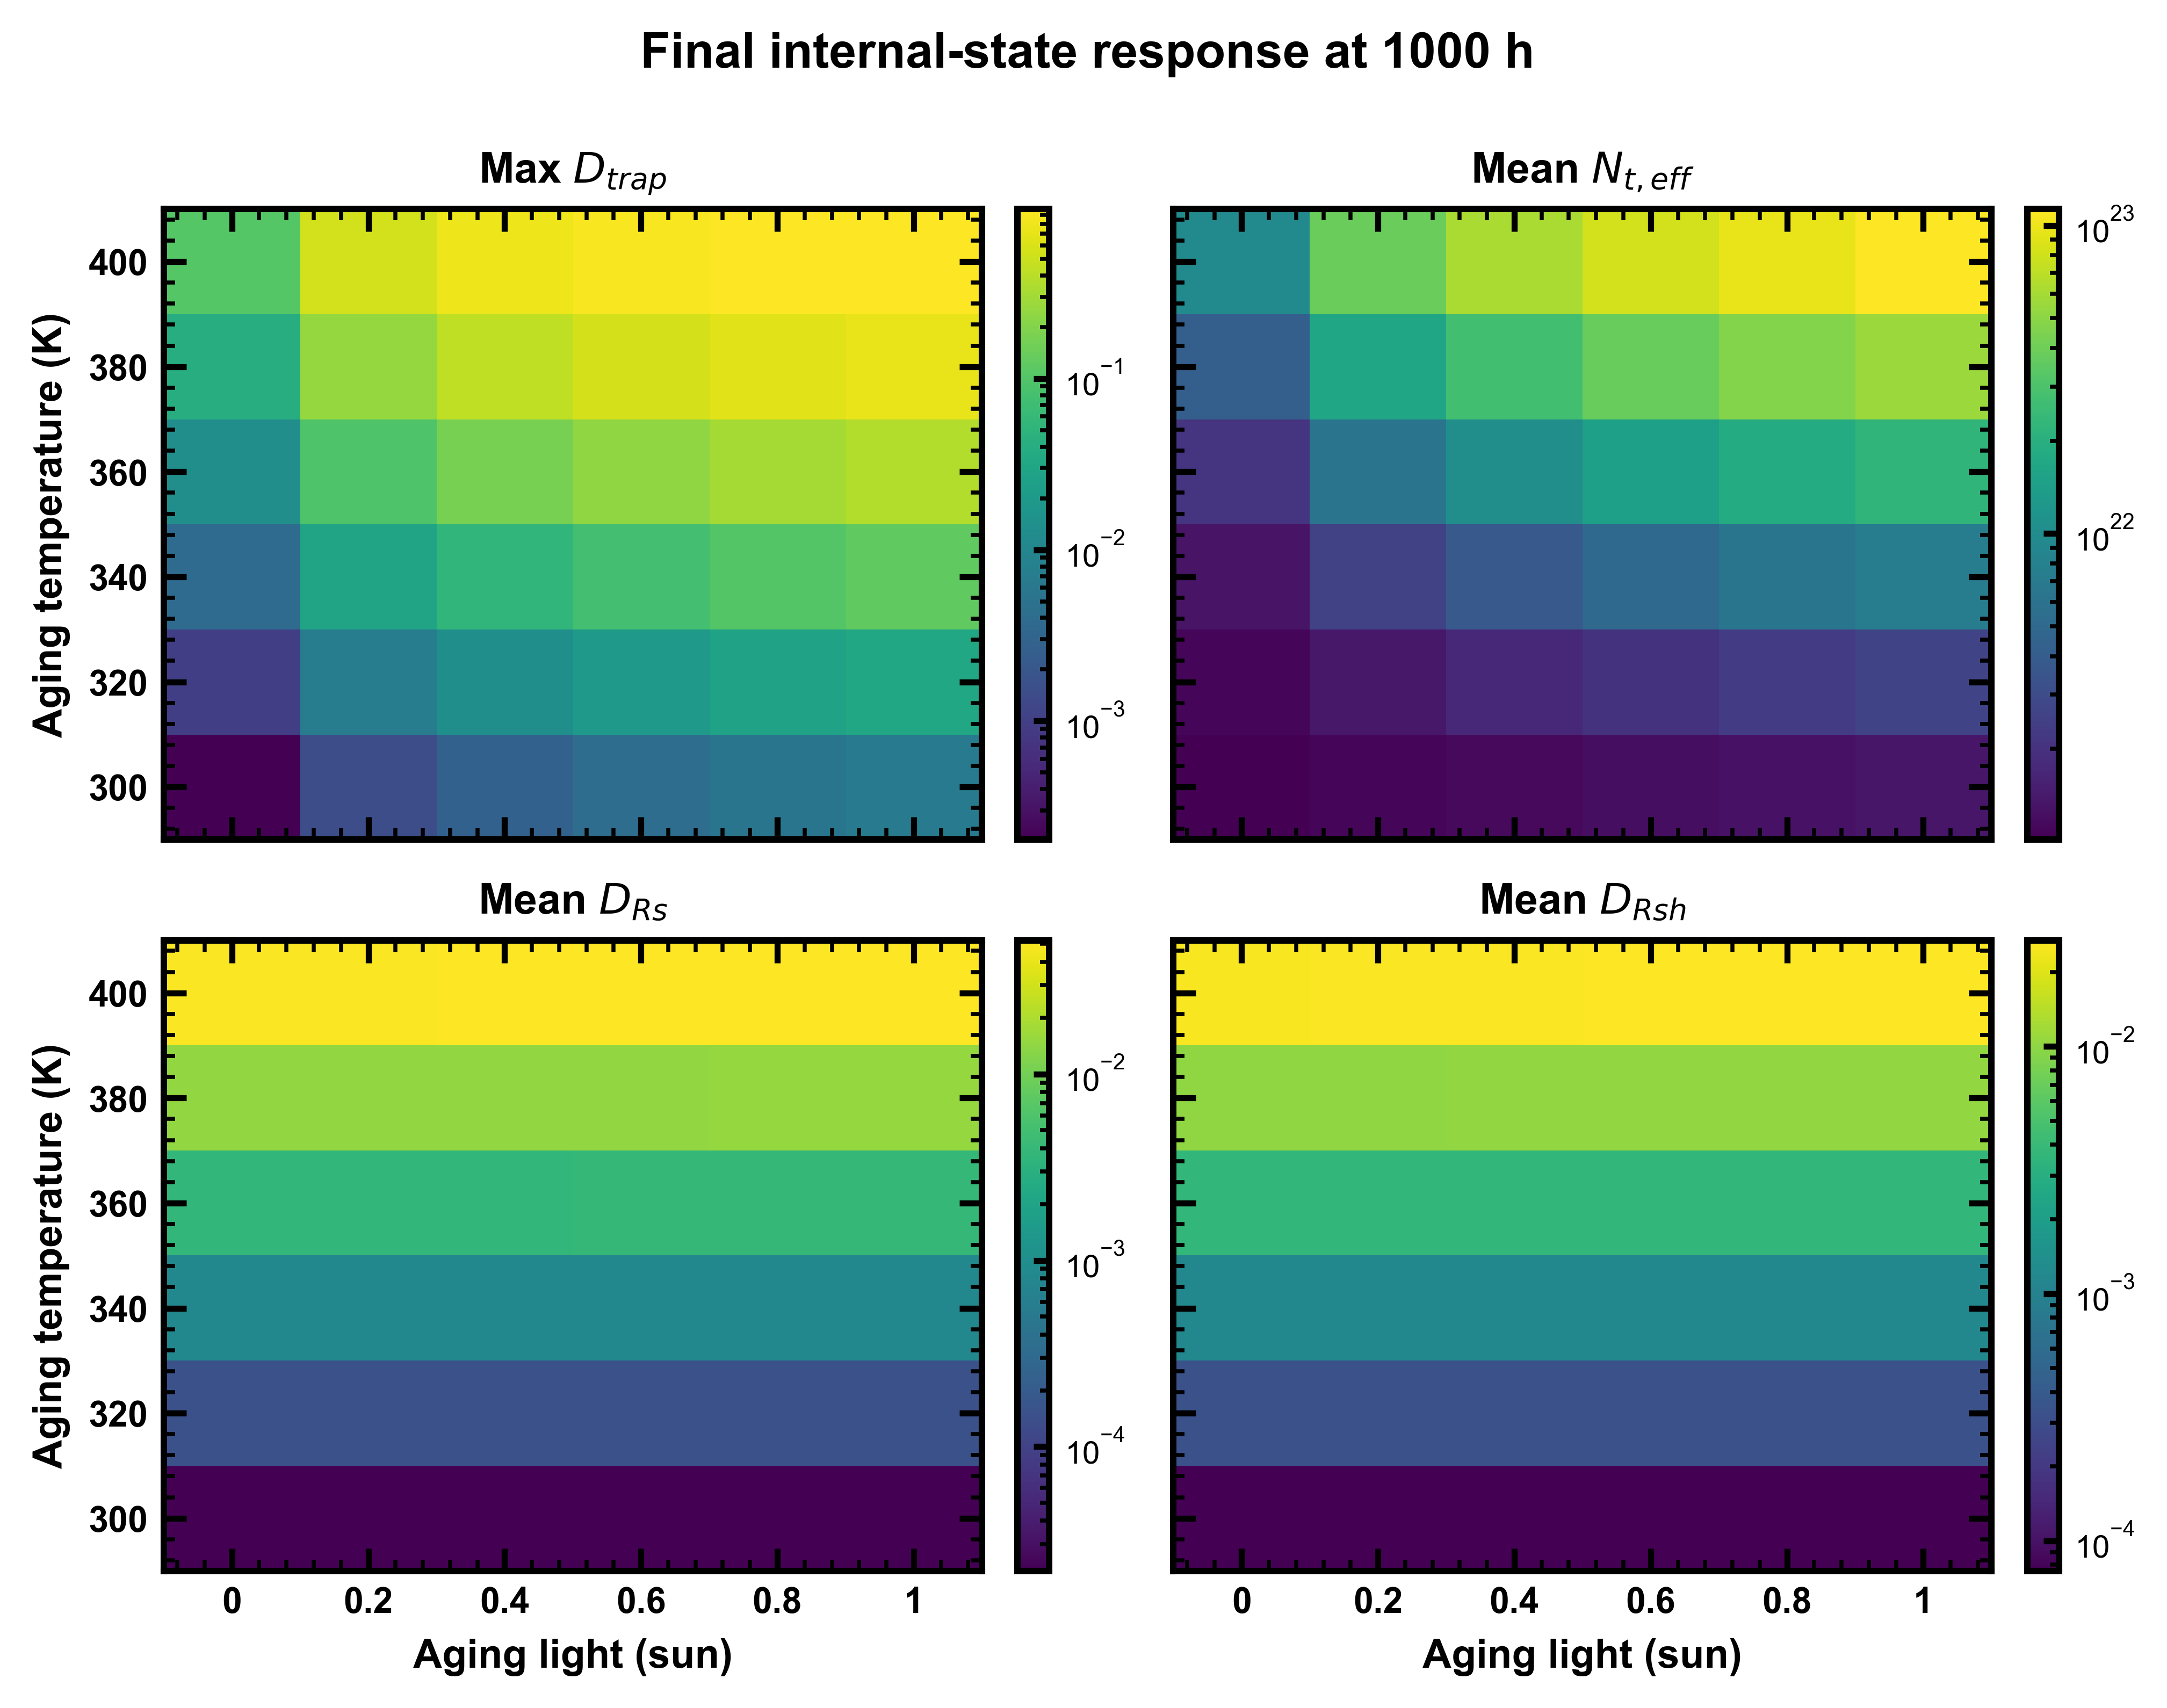
\includegraphics[width=\textwidth]{outputs/figures/comsol_architecture_stress_grid/profile_grid_final_state_summary.png}
\caption{Final 1000 h internal-state response from the baseline p-i-n 6 $\times$ 6 light-temperature profile grid. Trap damage and effective trap density increase with both light and temperature, while the resistance-damage states are dominated mainly by the temperature axis in this export.}
\label{fig:profile_grid_final_state_summary}
\end{figure}

\begin{table}[H]
\centering
\caption{Final 1000 h extrema from the baseline p-i-n light-temperature profile grid. The table reports where each state summary is smallest and largest across the 6 $\times$ 6 stress grid.}
\label{tab:profile_grid_extrema}
\begin{tabular}{@{}lrrrrrr@{}}
\toprule
State summary & Min & $T$ (K) & Light & Max & $T$ (K) & Light \\
\midrule
max $D_{\mathrm{trap}}$ & 0.000204 & 300 & 0 & 0.975 & 400 & 1 \\
max $u_{\mathrm{ion}}$ & 59 & 400 & 1 & 77.2 & 300 & 0 \\
mean $D_{Rs}$ & 2.16e-05 & 300 & 1 & 0.0522 & 400 & 1 \\
mean $D_{Rsh}$ & 7.57e-05 & 300 & 1 & 0.0268 & 400 & 1 \\
mean $N_{t,\mathrm{eff}}$ & 1.02e+21 & 300 & 0 & 1.13e+23 & 400 & 1 \\
\bottomrule
\end{tabular}
\end{table}


Figure~\ref{fig:profile_grid_final_state_summary} and
Table~\ref{tab:profile_grid_extrema} show the expected stress ordering for the
irreversible trap and resistance-damage states. The smallest final trap
response occurs at the lowest light and temperature, while the largest final
trap and effective trap-density responses occur at 400 K and one sun. The
resistance-damage states increase by orders of magnitude with temperature but
are comparatively weakly dependent on light in this parameterization. The
maximum mobile-ion accumulation should be interpreted differently: it is a
redistribution diagnostic controlled by electric field, thermal voltage, and
preconditioning state, not a monotonic irreversible damage variable. This
distinction is useful for future inverse modeling: a terminal J--V curve alone
may not separate trap growth from resistance evolution, but a COMSOL-generated
state grid can define the physically plausible state manifold for surrogate
training.

\section{Lite COMSOL-Trained Surrogate Baseline}

The validated light-temperature J--V export and profile-grid summaries also
define the first traceable machine-learning data product in the thesis. The
purpose of this section is limited: it tests whether the current COMSOL export
contract can support a forward surrogate with scenario-held-out validation. It
does not claim a final experimentally calibrated digital twin, and it does not
train an inverse model from measured data. The reproducible entry point is
\path{scripts/train_lite_surrogates.py}, which reads the processed COMSOL
tables, encodes the stored 0.01-sun numerical floor as the displayed 0-sun
condition, trains lightweight random-forest baselines, and writes model files,
validation predictions, figures, tables, and metadata under
\path{models/surrogate_lite/},
\path{outputs/figures/surrogate_lite/}, and
\path{outputs/tables/surrogate_lite/}.

\begin{figure}[H]
\centering
\begin{minipage}{0.49\textwidth}
\centering
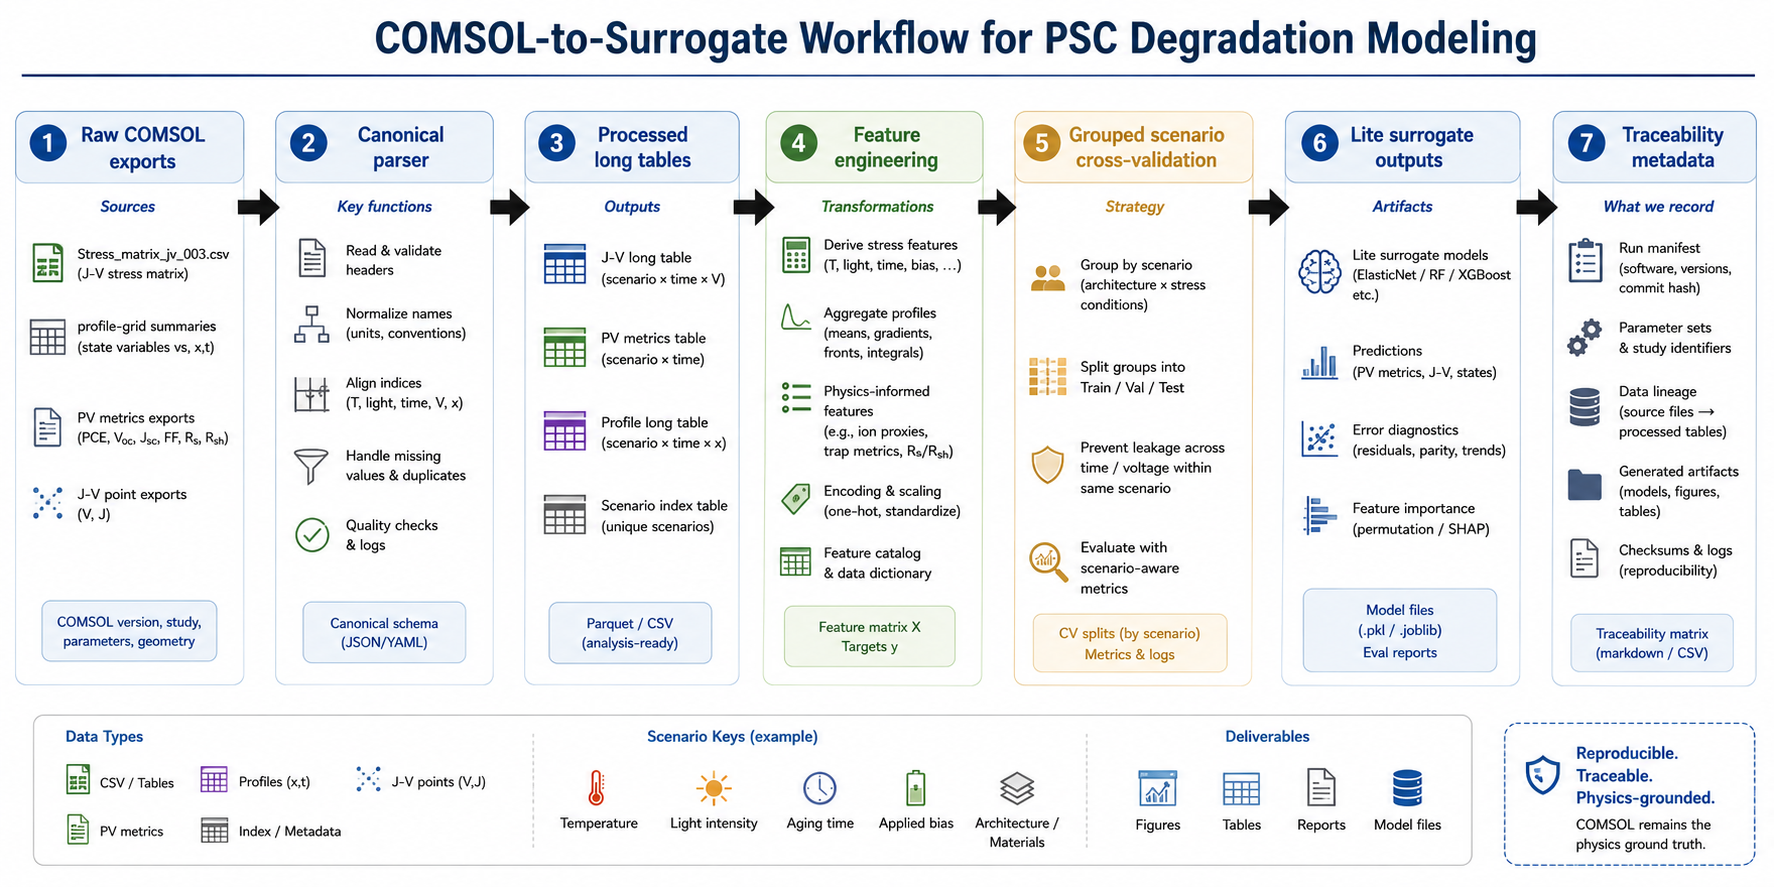
\includegraphics[width=\textwidth]{figures/ml_surrogate/comsol_to_surrogate_workflow_concept.png}
\end{minipage}\hfill
\begin{minipage}{0.49\textwidth}
\centering
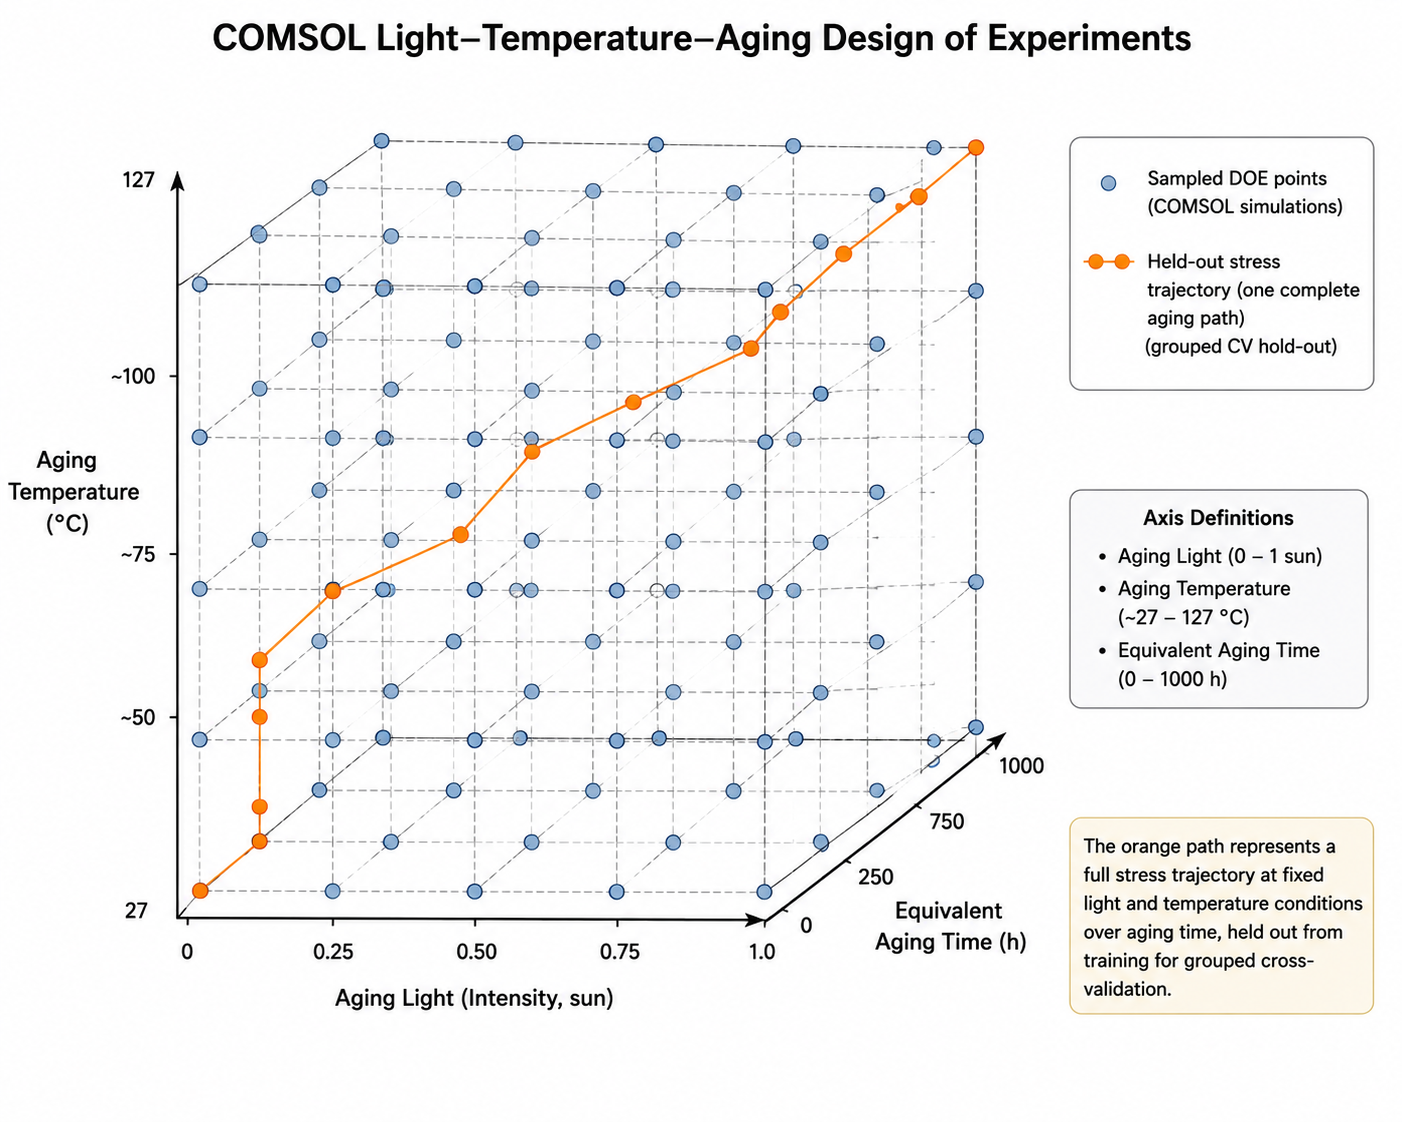
\includegraphics[width=\textwidth]{figures/ml_surrogate/aging_doe_trajectory_concept.png}
\end{minipage}
\caption[Conceptual COMSOL-to-ML workflow and design-of-experiments map.]{Conceptual schematics for the COMSOL-to-ML workflow and the
light-temperature-aging design of experiments. These panels summarize the data
contract and sampling logic; quantitative validation results are generated
separately by the reproducible surrogate scripts.}
\label{fig:ml_concept_workflow_doe}
\end{figure}

\begin{figure}[H]
\centering
\begin{minipage}{0.49\textwidth}
\centering
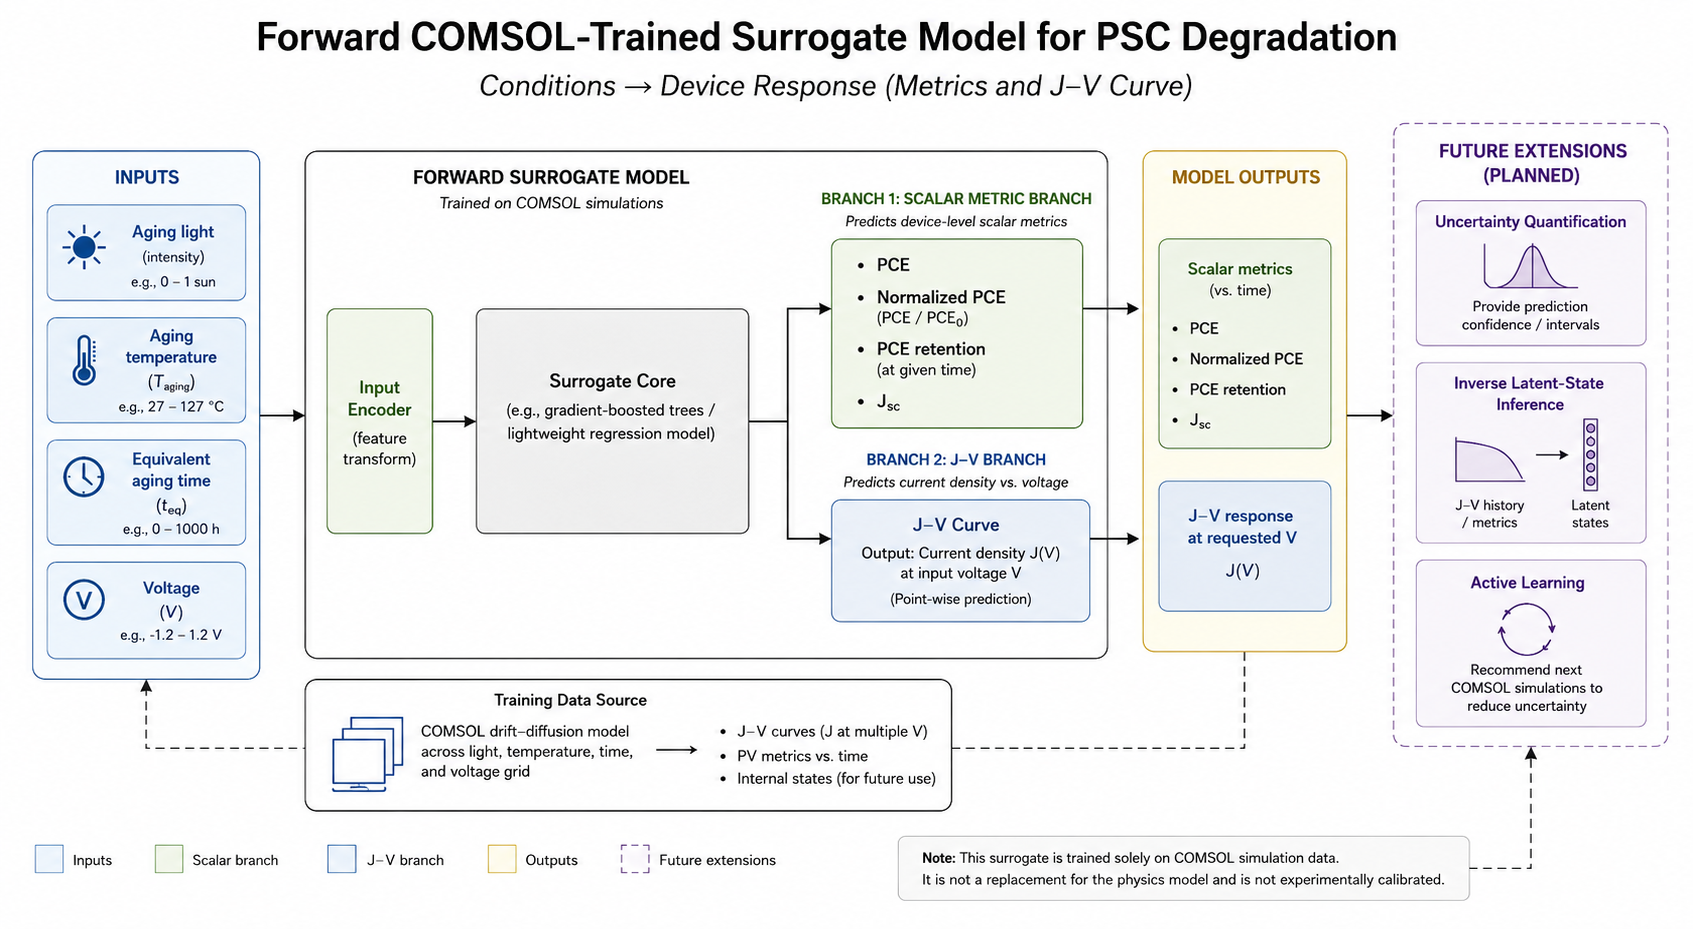
\includegraphics[width=\textwidth]{figures/ml_surrogate/forward_surrogate_architecture_concept.png}
\end{minipage}\hfill
\begin{minipage}{0.49\textwidth}
\centering
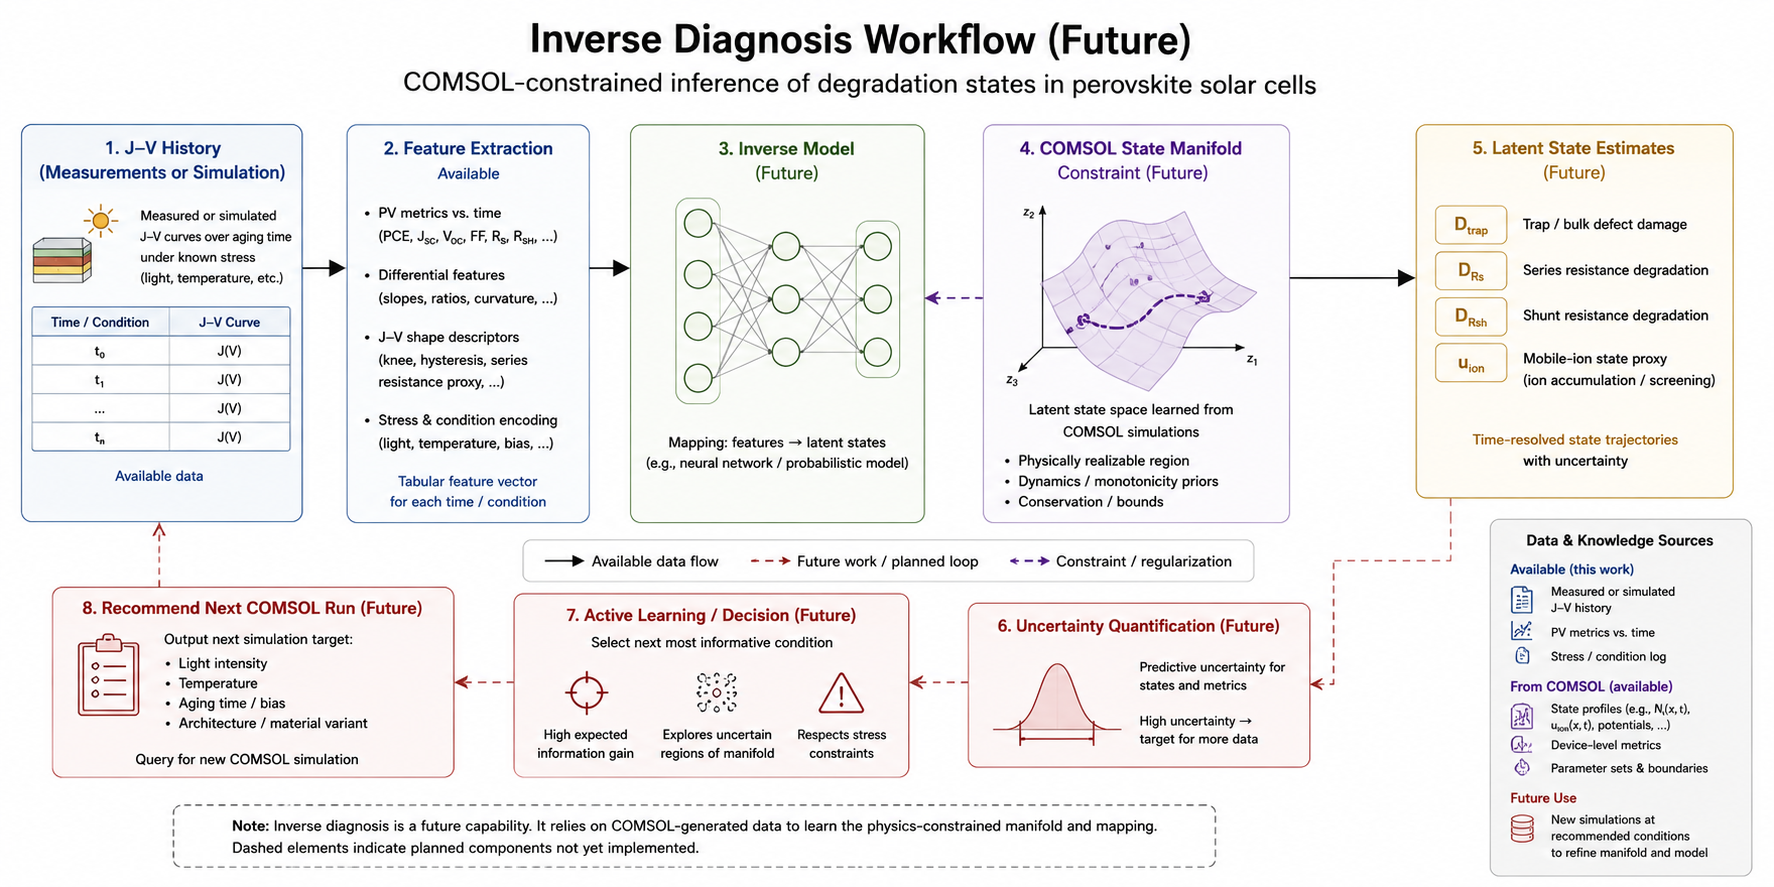
\includegraphics[width=\textwidth]{figures/ml_surrogate/inverse_diagnosis_workflow_concept.png}
\end{minipage}
\caption[Conceptual forward-surrogate and inverse-diagnosis architecture.]{Conceptual architecture diagrams for the forward COMSOL-trained
surrogate and the future inverse-diagnosis workflow. The present thesis trains
and validates the forward lite surrogate only; inverse diagnosis remains a
planned extension requiring broader COMSOL state labels and experimental
calibration.}
\label{fig:ml_concept_forward_inverse}
\end{figure}

\begin{figure}[H]
\centering
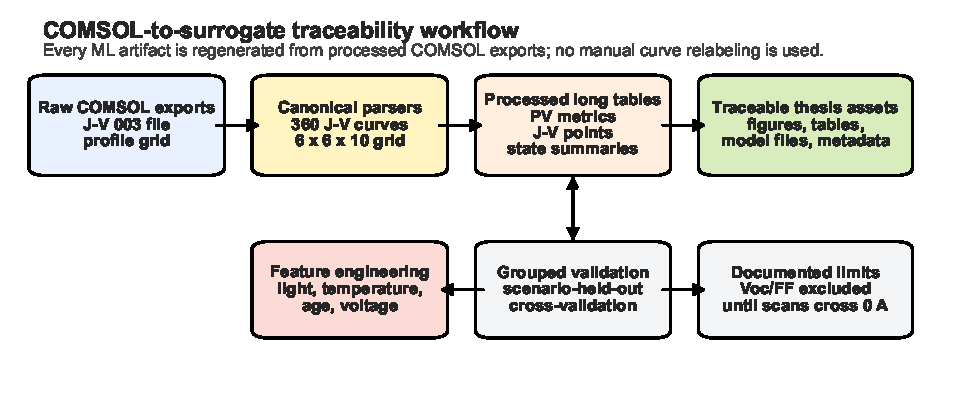
\includegraphics[width=\textwidth]{outputs/figures/surrogate_lite/surrogate_lite_data_traceability_workflow.pdf}
\caption{Traceable COMSOL-to-surrogate workflow for the lite ML baseline. The
raw flat J--V and profile-grid exports are parsed into long tables, converted
into stress, age, and voltage features, evaluated with scenario-held-out
cross-validation, and written as auditable thesis artifacts.}
\label{fig:surrogate_lite_traceability}
\end{figure}

The current ML-ready data set contains 36 light-temperature scenarios, ten
aging checkpoints per scenario, and 48 voltage samples per J--V curve, giving
360 diagnostic curves and 17,280 current-density points. The profile-grid
summary contributes 2520 internal-state rows across seven exported variables.
The voltage sweep ends at 1.25 V, so only 115 of the 360 curves have resolved
zero-current crossings. For this reason, $V_{oc}$ and FF are excluded from the
lite surrogate targets until the diagnostic voltage range is extended. The
trained scalar targets are PCE, normalized PCE, PCE retention, and $J_{sc}$;
the curve target is current density $J(V)$.

\begin{table}[H]
\centering
\caption{Grouped scenario cross-validation metrics for the lite COMSOL-trained surrogate baseline. Scenario grouping keeps complete light-temperature aging trajectories out of the training fold before prediction.}
\label{tab:surrogate_lite_cv_metrics}
\begin{tabular}{@{}lrrrr@{}}
\toprule
Target & Samples & Groups & MAE & $R^2$ \\
\midrule
PCE (%) & 360 & 36 & 0.393 & 0.884 \\
Normalized PCE $(\mathrm{PCE}/\mathrm{PCE}_0)$ & 360 & 36 & 0.0174 & 0.884 \\
PCE retention (%) & 360 & 36 & 1.74 & 0.884 \\
$J_{sc}$ (mA cm$^{-2}$) & 360 & 36 & 0.0767 & 0.864 \\
$J(V)$ (mA cm$^{-2}$) & 17280 & 36 & 0.286 & 0.955 \\
\bottomrule
\end{tabular}
\end{table}


\begin{figure}[H]
\centering
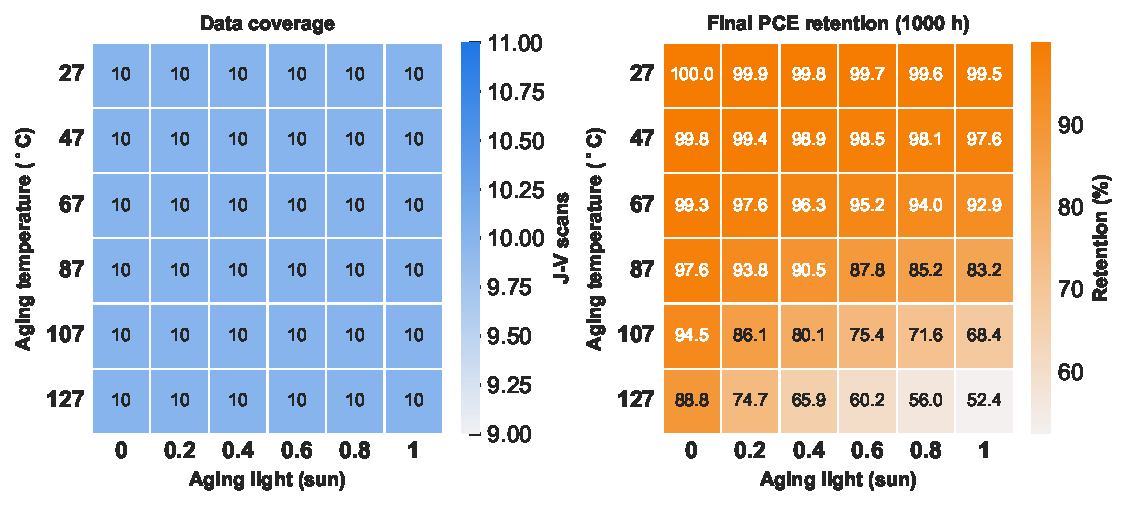
\includegraphics[width=0.95\textwidth]{outputs/figures/surrogate_lite/surrogate_lite_doe_coverage.pdf}
\caption{Design-of-experiments coverage and final degradation surface used for
the lite surrogate. Each light-temperature scenario has ten diagnostic J--V
curves, and the final PCE-retention surface spans near-unity retention at low
stress to 52.4\% at 400 K and one sun.}
\label{fig:surrogate_lite_doe_coverage}
\end{figure}

\begin{figure}[H]
\centering
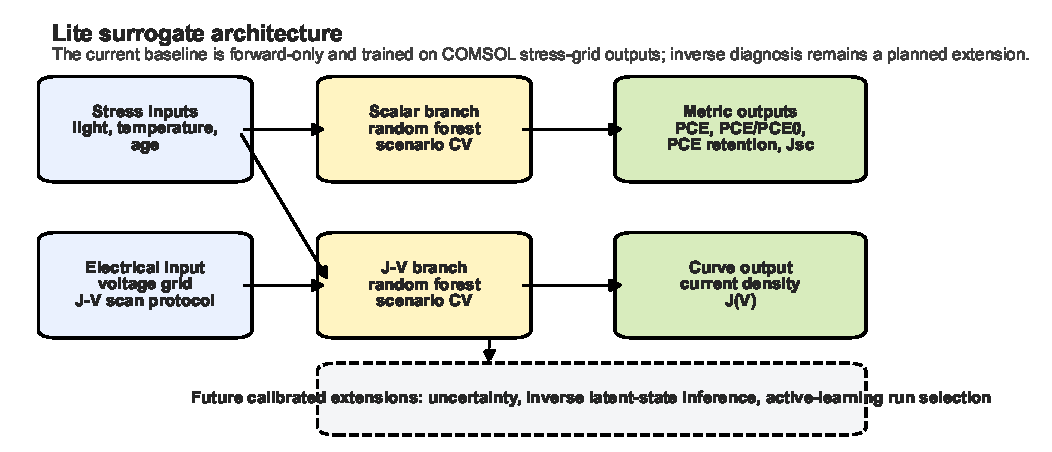
\includegraphics[width=\textwidth]{outputs/figures/surrogate_lite/surrogate_lite_model_architecture.pdf}
\caption{Forward surrogate architecture used for the lite baseline. Stress and
age features feed scalar photovoltaic metric models, while stress, age, and
voltage feed the J--V current-density model. Uncertainty, inverse diagnosis,
and active learning remain planned calibrated extensions.}
\label{fig:surrogate_lite_architecture}
\end{figure}

The validation split is grouped by \texttt{scenario\_index}. Entire
light-temperature aging trajectories are held out by fold rather than randomly
mixing rows from the same scenario into training and test sets. This is a more
conservative test of interpolation across stress space. Table
\ref{tab:surrogate_lite_cv_metrics} shows that the first baseline already
predicts PCE retention with 1.74 percentage-point MAE and predicts
current-density points with $0.286~\mathrm{mA/cm^2}$ MAE. The scalar $R^2$
values are about 0.86--0.88, while the J--V current-density model reaches
$R^2=0.955$. These values are promising for a lightweight surrogate, but they
should be interpreted as COMSOL-to-COMSOL interpolation accuracy, not
experimental prediction accuracy.

\begin{figure}[H]
\centering
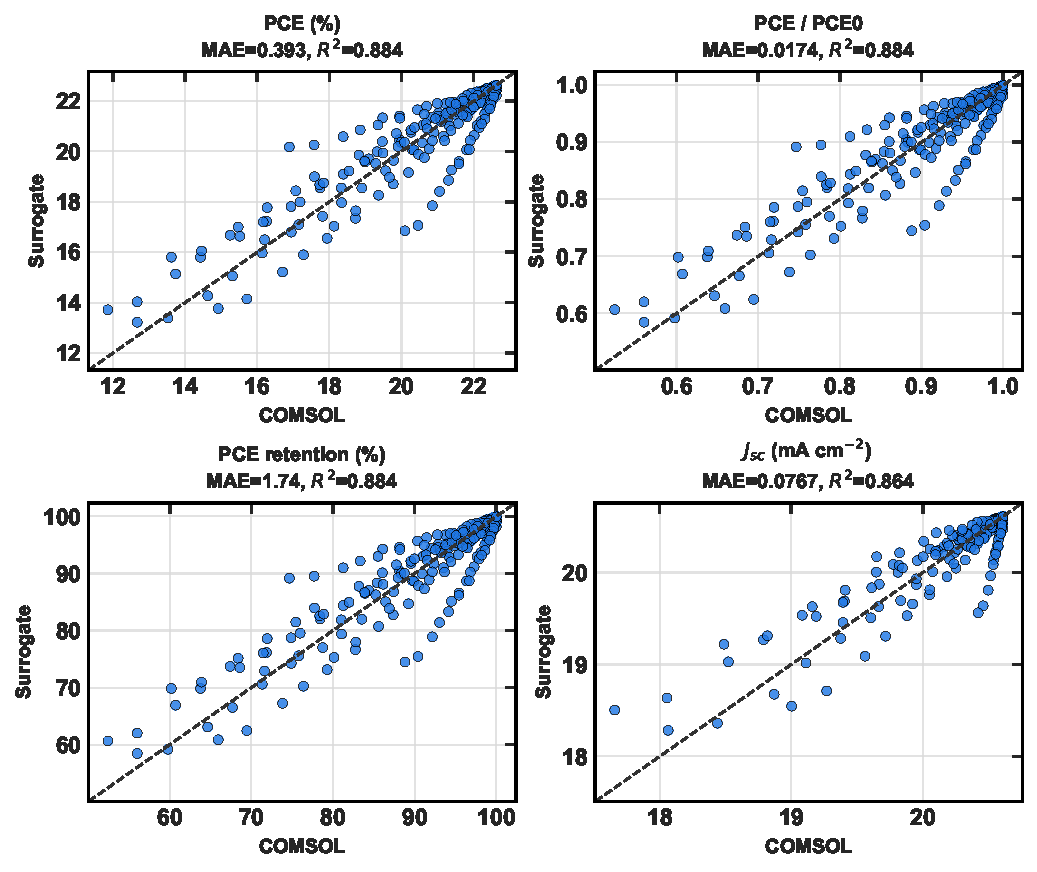
\includegraphics[width=0.92\textwidth]{outputs/figures/surrogate_lite/surrogate_lite_actual_vs_pred.pdf}
\caption{Scenario-held-out COMSOL versus lite-surrogate predictions for scalar
photovoltaic targets. The diagonal line is the ideal one-to-one response.}
\label{fig:surrogate_lite_actual_vs_pred}
\end{figure}

\begin{figure}[H]
\centering
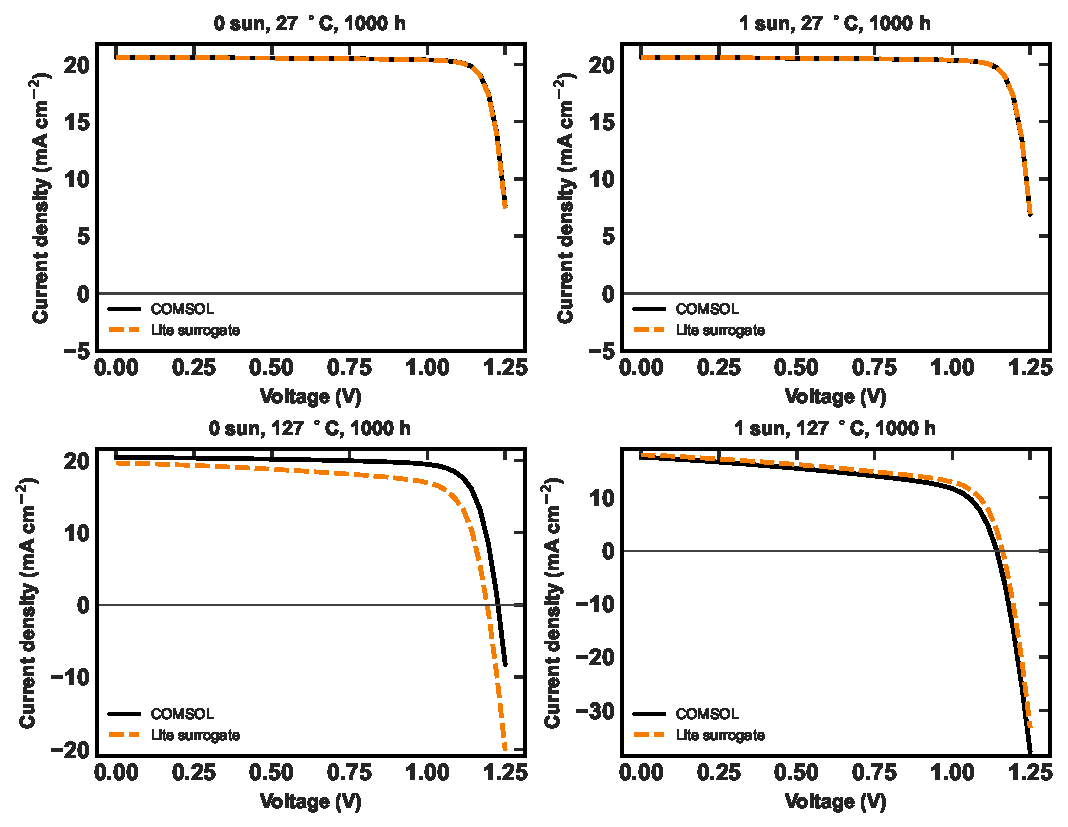
\includegraphics[width=0.92\textwidth]{outputs/figures/surrogate_lite/surrogate_lite_jv_group_cv_examples.pdf}
\caption[Scenario-held-out J--V examples for the lite surrogate.]{Representative scenario-held-out J--V predictions at the four
light-temperature stress corners after 1000 h equivalent aging. The
low-stress corners remain close to the COMSOL curves, while the high-temperature
corners expose the largest interpolation errors near the knee and zero-current
region.}
\label{fig:surrogate_lite_jv_examples}
\end{figure}

\begin{figure}[H]
\centering
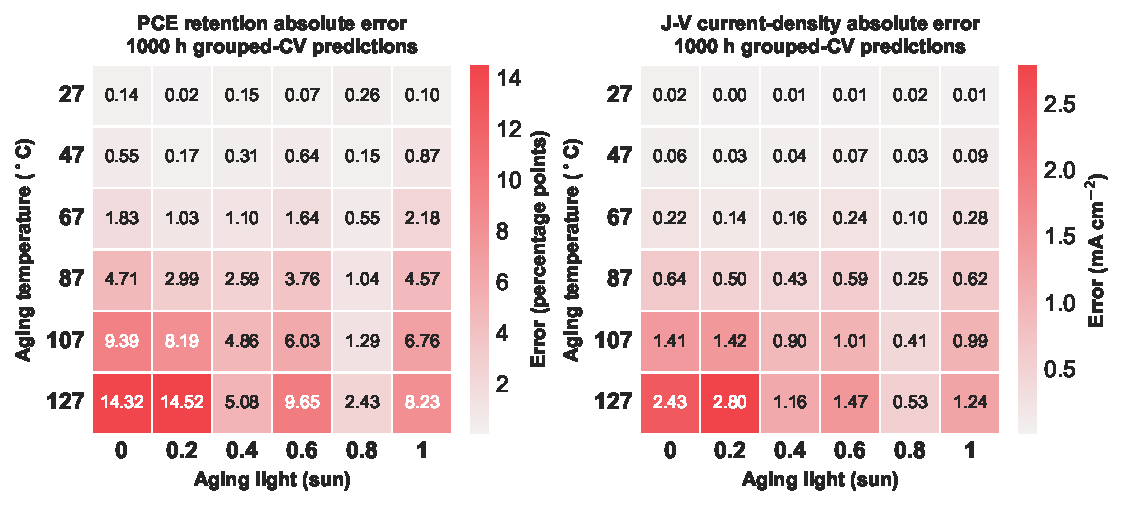
\includegraphics[width=0.95\textwidth]{outputs/figures/surrogate_lite/surrogate_lite_error_maps.pdf}
\caption{Final-age absolute-error maps from the grouped cross-validation
predictions. The largest PCE-retention errors occur at the highest-temperature
edge of the stress grid, identifying where additional COMSOL simulations or a
more structured surrogate would be most useful.}
\label{fig:surrogate_lite_error_maps}
\end{figure}

\begin{figure}[H]
\centering
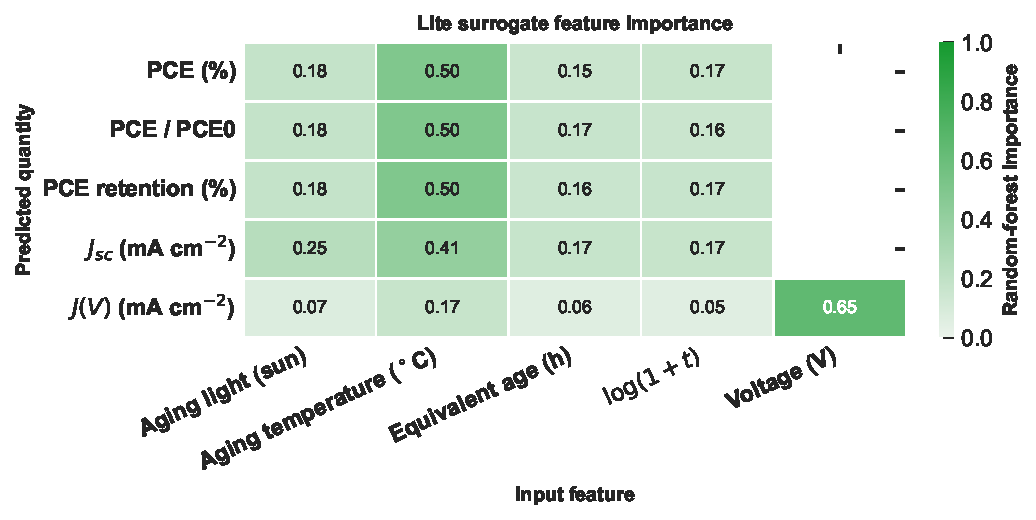
\includegraphics[width=0.86\textwidth]{outputs/figures/surrogate_lite/surrogate_lite_feature_importance.pdf}
\caption{Random-forest feature importances for the final lite surrogate models.
Temperature dominates the scalar degradation targets in this COMSOL export,
while voltage dominates the J--V current-density branch as expected.}
\label{fig:surrogate_lite_feature_importance}
\end{figure}

\begin{figure}[H]
\centering
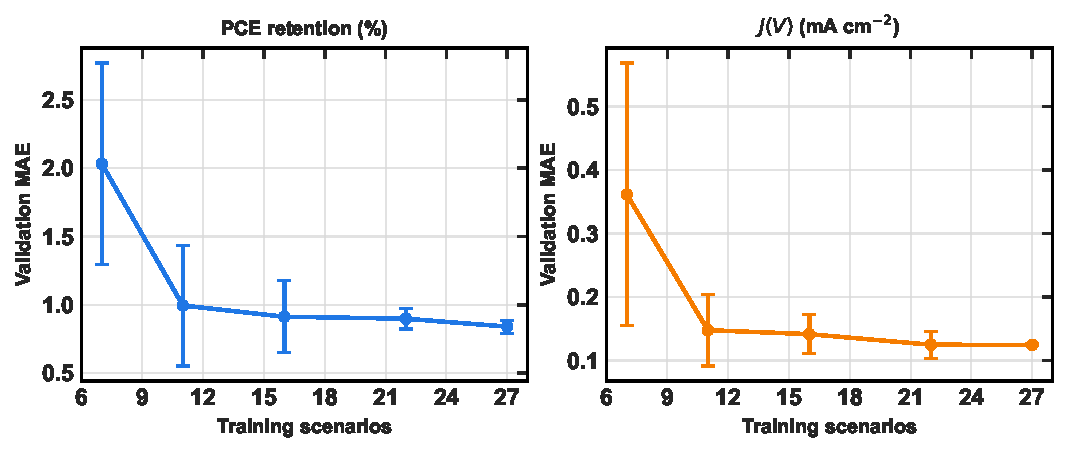
\includegraphics[width=0.84\textwidth]{outputs/figures/surrogate_lite/surrogate_lite_learning_curve.pdf}
\caption{Training-size sensitivity for the lite surrogate. The validation MAE
drops rapidly after the smallest training subsets and then begins to plateau,
indicating that the existing grid is enough for a first baseline but not enough
to replace calibrated COMSOL sweeps.}
\label{fig:surrogate_lite_learning_curve}
\end{figure}

The ML result is therefore a useful thesis support result. It proves that the
COMSOL exports can be converted into a reproducible surrogate-ready data set,
that grouped validation is possible without manual relabeling, and that the
largest residuals can be traced back to specific stress regions. The remaining
gap is calibration and breadth: future work should add more architectures,
complete voltage windows for $V_{oc}$ and FF, repeated COMSOL samples for
uncertainty, and matched experimental aging data before the surrogate is used
for inverse diagnosis or field prediction.

\section{Current Data-Quality Gaps}

The canonical light-temperature stress-matrix J--V result in this thesis is
\path{data/raw/comsol/arch_baseline_pin/Aging/Stress_matrix_jv_003.csv}. Earlier
exports, \path{Stress_matrix_jv_001.csv} and \path{Stress_matrix_jv_002.csv},
are retained only as superseded development history. They are useful for
auditing the export evolution, but they should not be interpreted as missing
low-light data or as parallel quantitative results. The current remaining
data-quality limitation is instead the voltage range of the canonical
\path{Stress_matrix_jv_003.csv} export: many mild or early-aging curves do not
cross zero current by 1.25 V. Therefore PCE and $J_{sc}$ are available for the
full 360-curve grid, while $V_{oc}$ and FF are complete only for the subset of
curves with a resolved zero-current crossing. A future diagnostic sweep to
approximately 1.45 V would make $V_{oc}$ and FF complete across the full
light-temperature grid.

\section{Hysteresis Result}

\begin{figure}[H]
\centering
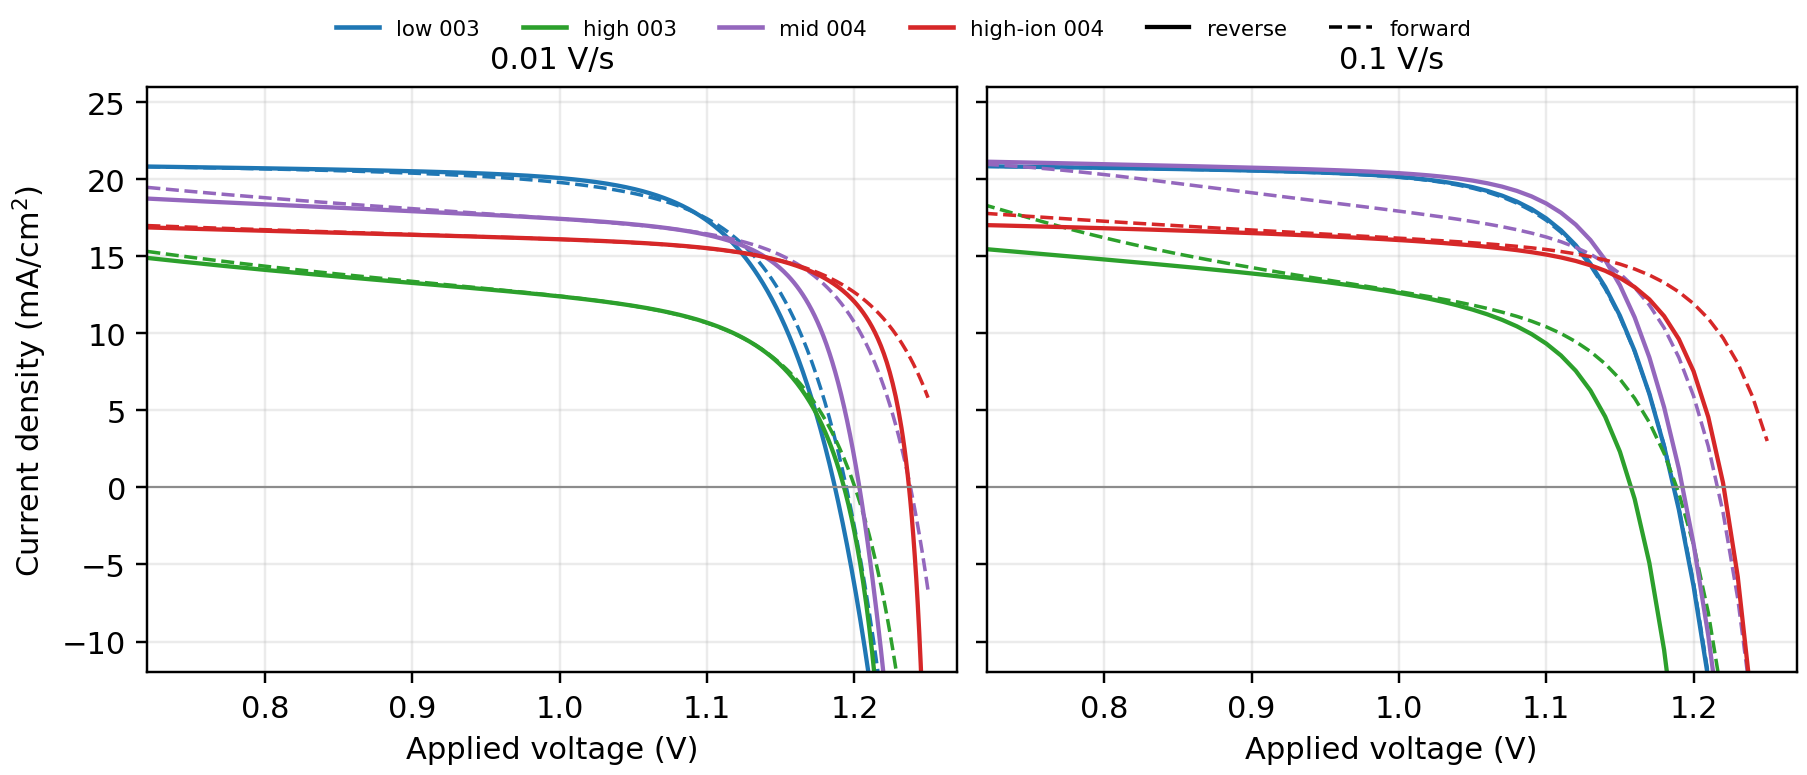
\includegraphics[width=0.78\textwidth]{figures/eee598_comsol/jv_curves.png}
\caption{Forward and reverse J--V scans from the COMSOL hysteresis protocol.}
\label{fig:results_hysteretic_jv}
\end{figure}

Figure~\ref{fig:results_hysteretic_jv} shows scan-direction-dependent J--V
behavior. The variable that changes during the scan is the normalized ion state
$u_{\mathrm{ion}}$. Through Eq.~\ref{eq:rho_ion}, ion redistribution modifies
the electrostatic source term. As ions accumulate near one interface and
deplete near the opposite side, the internal charge distribution changes,
altering band bending and shifting the measured J--V curve depending on scan
history. The result supports the physical need for time-dependent scan
simulation. This presentation case uses
$N_0=10^{17}~\mathrm{cm^{-3}}$,
$\mu_{\mathrm{ion}}=10^{-18}~\mathrm{m^2/(V\,s)}$, and
$r_{\mathrm{scan}}=0.1~\mathrm{V/s}$. It is a separate presentation diagnostic
case rather than part of the canonical
\path{Stress_matrix_jv_003.csv} light-temperature grid, and it does not prove
that the selected ion mobility or concentration is unique.

\section{Spatial and Transient Validation Results}

The newest COMSOL profile exports include the band-edge and quasi-Fermi-level
variables needed to check the simulated internal electrostatics. The selected
band-diagram cases in Fig.~\ref{fig:band_diagrams_selected_cases} use the
native left-to-right COMSOL coordinate, with the HTL side on the left and the
ETL side on the right. Energies were exported by COMSOL as joules and converted
to electron-volts for plotting. The resulting profiles show a monotonic
internal band-bending trend across the absorber and carrier-selective
alignment at the transport-layer sides. These plots do not replace a full
operating-point validation at short circuit, maximum power, and open circuit,
but they remove the previous coordinate-direction ambiguity.

\begin{figure}[H]
\centering
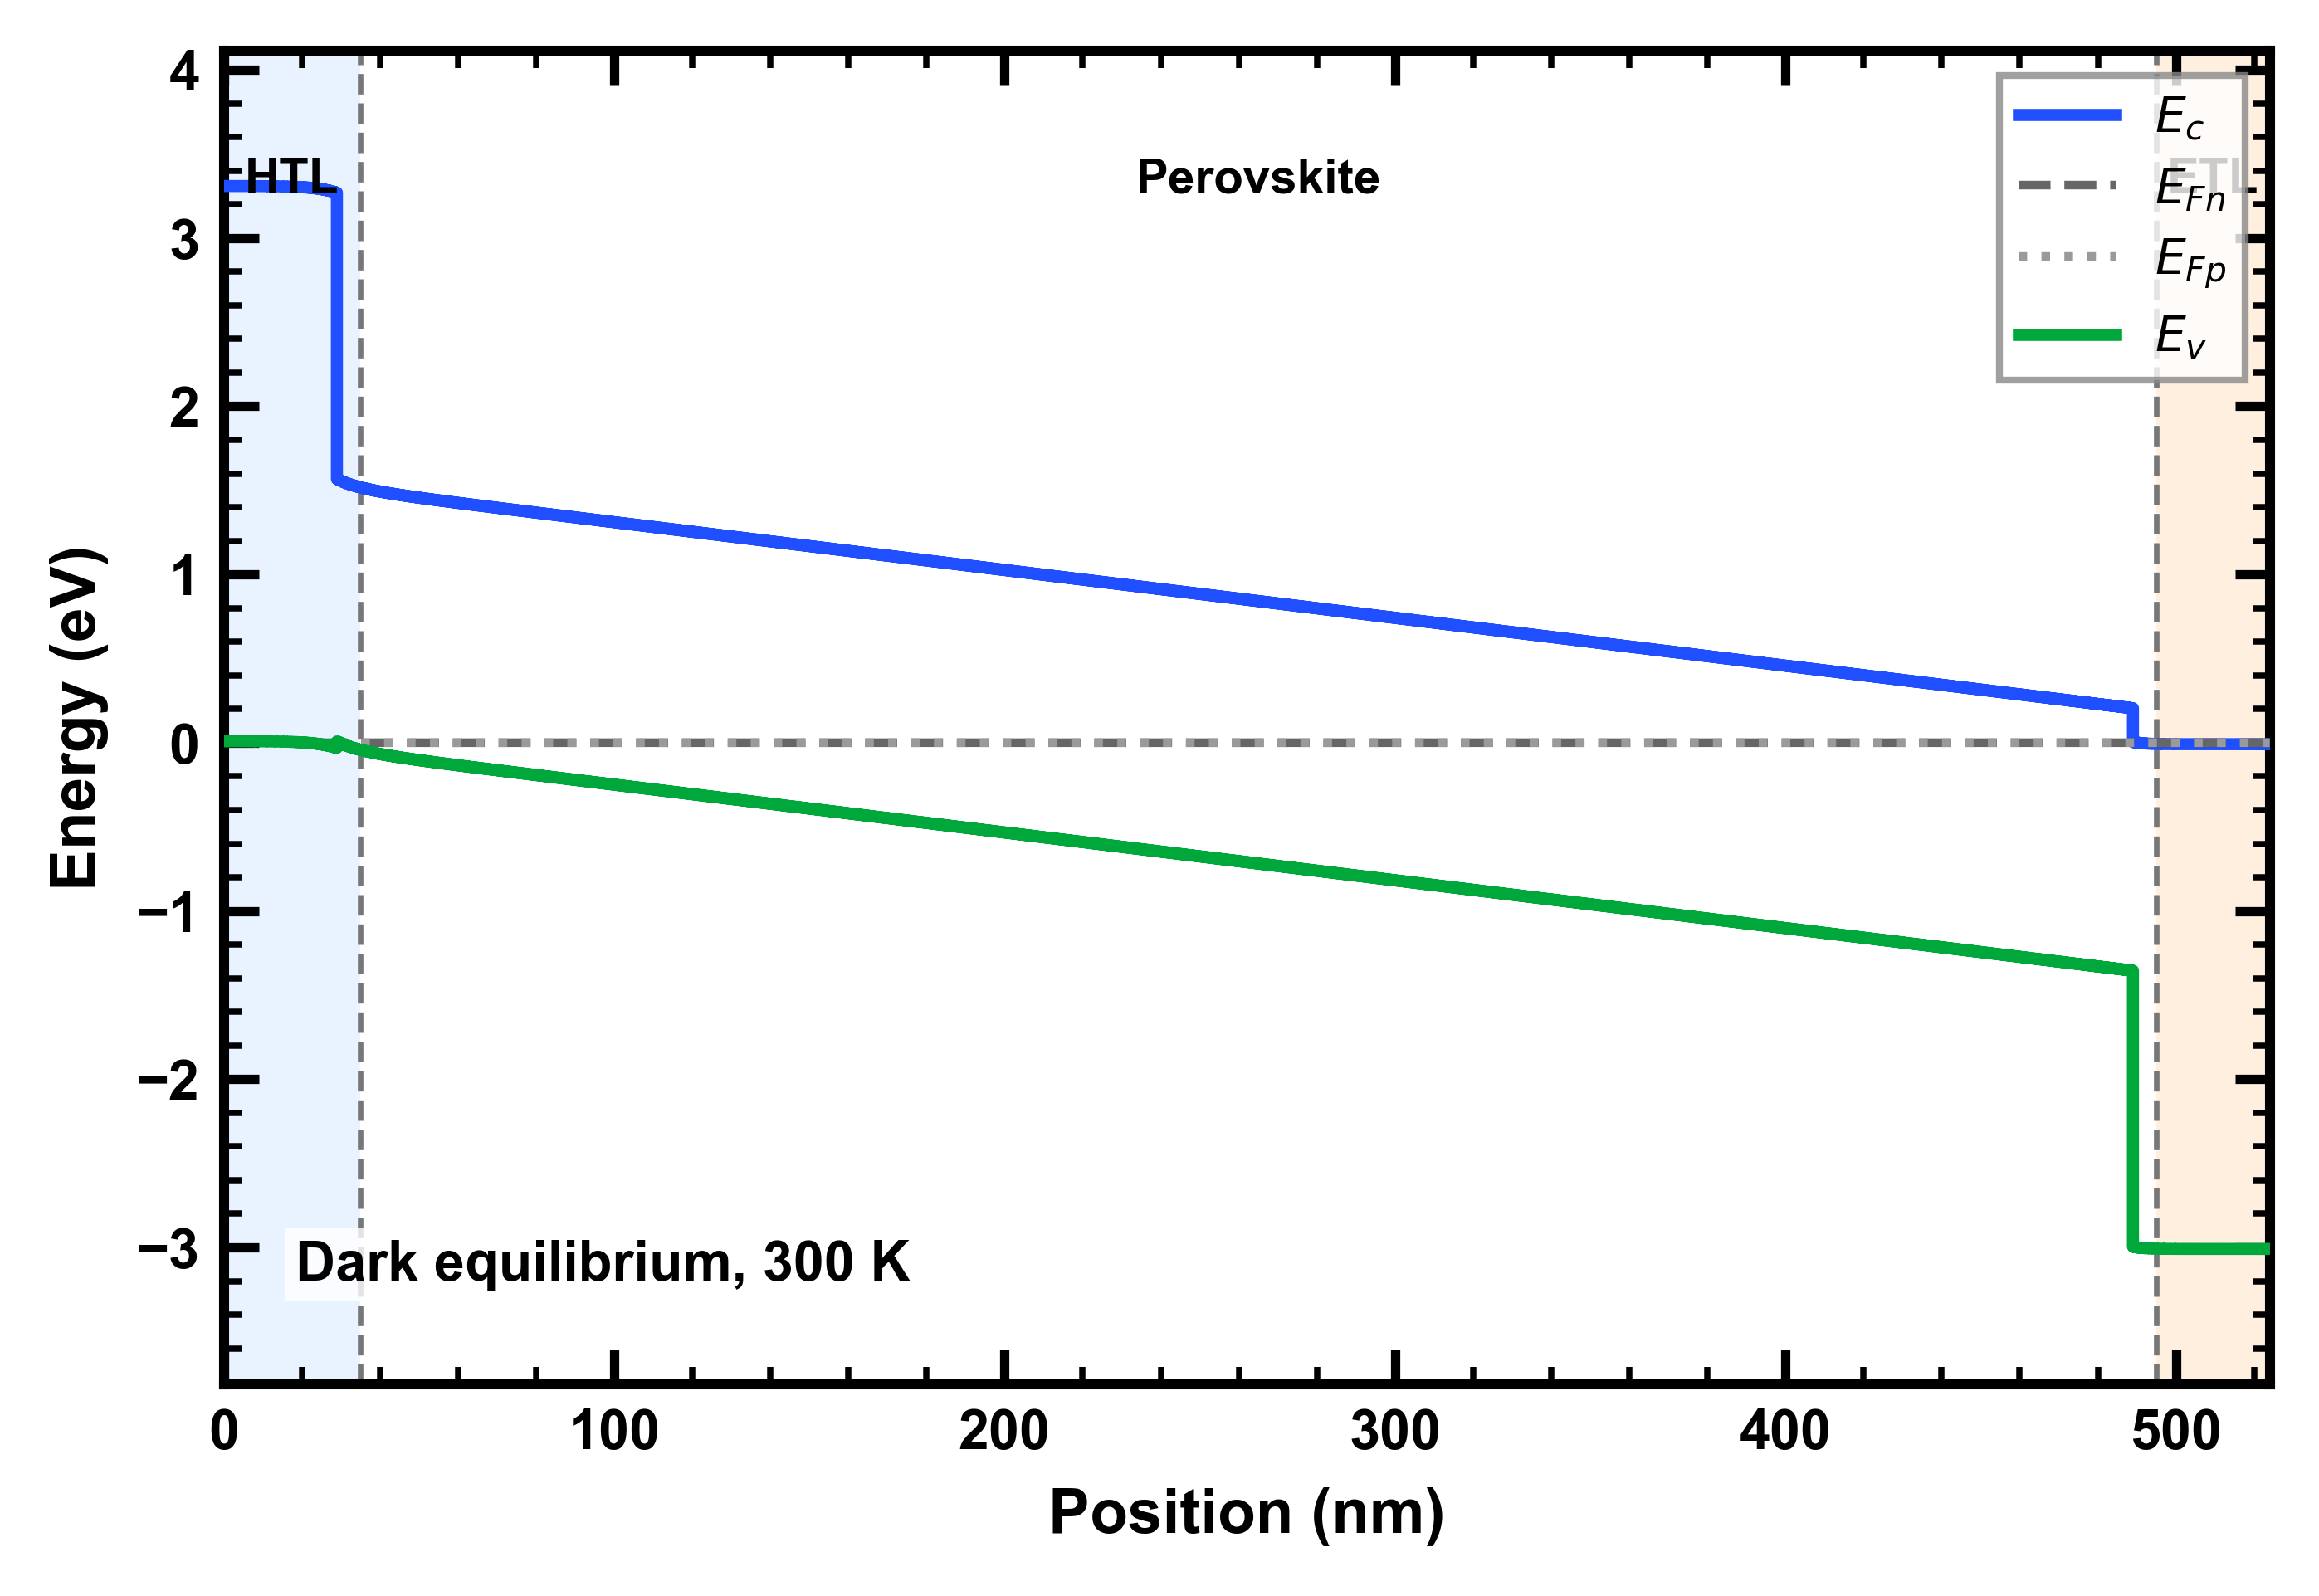
\includegraphics[width=0.76\textwidth]{outputs/figures/comsol_architecture_stress_grid/baseline_pin_band_diagram_dark_equilibrium_300K.png}
\caption{COMSOL dark-equilibrium band diagram for the 300 K baseline device.
This figure is generated from the dedicated equilibrium energy-level export,
not from the low-light aging grid. The electron and hole quasi-Fermi levels
overlap to numerical precision, as expected for a true equilibrium solution.
The native coordinate is preserved, with the HTL on the left and the ETL on the
right.}
\label{fig:band_diagram_dark_equilibrium_300k}
\end{figure}

\begin{figure}[H]
\centering
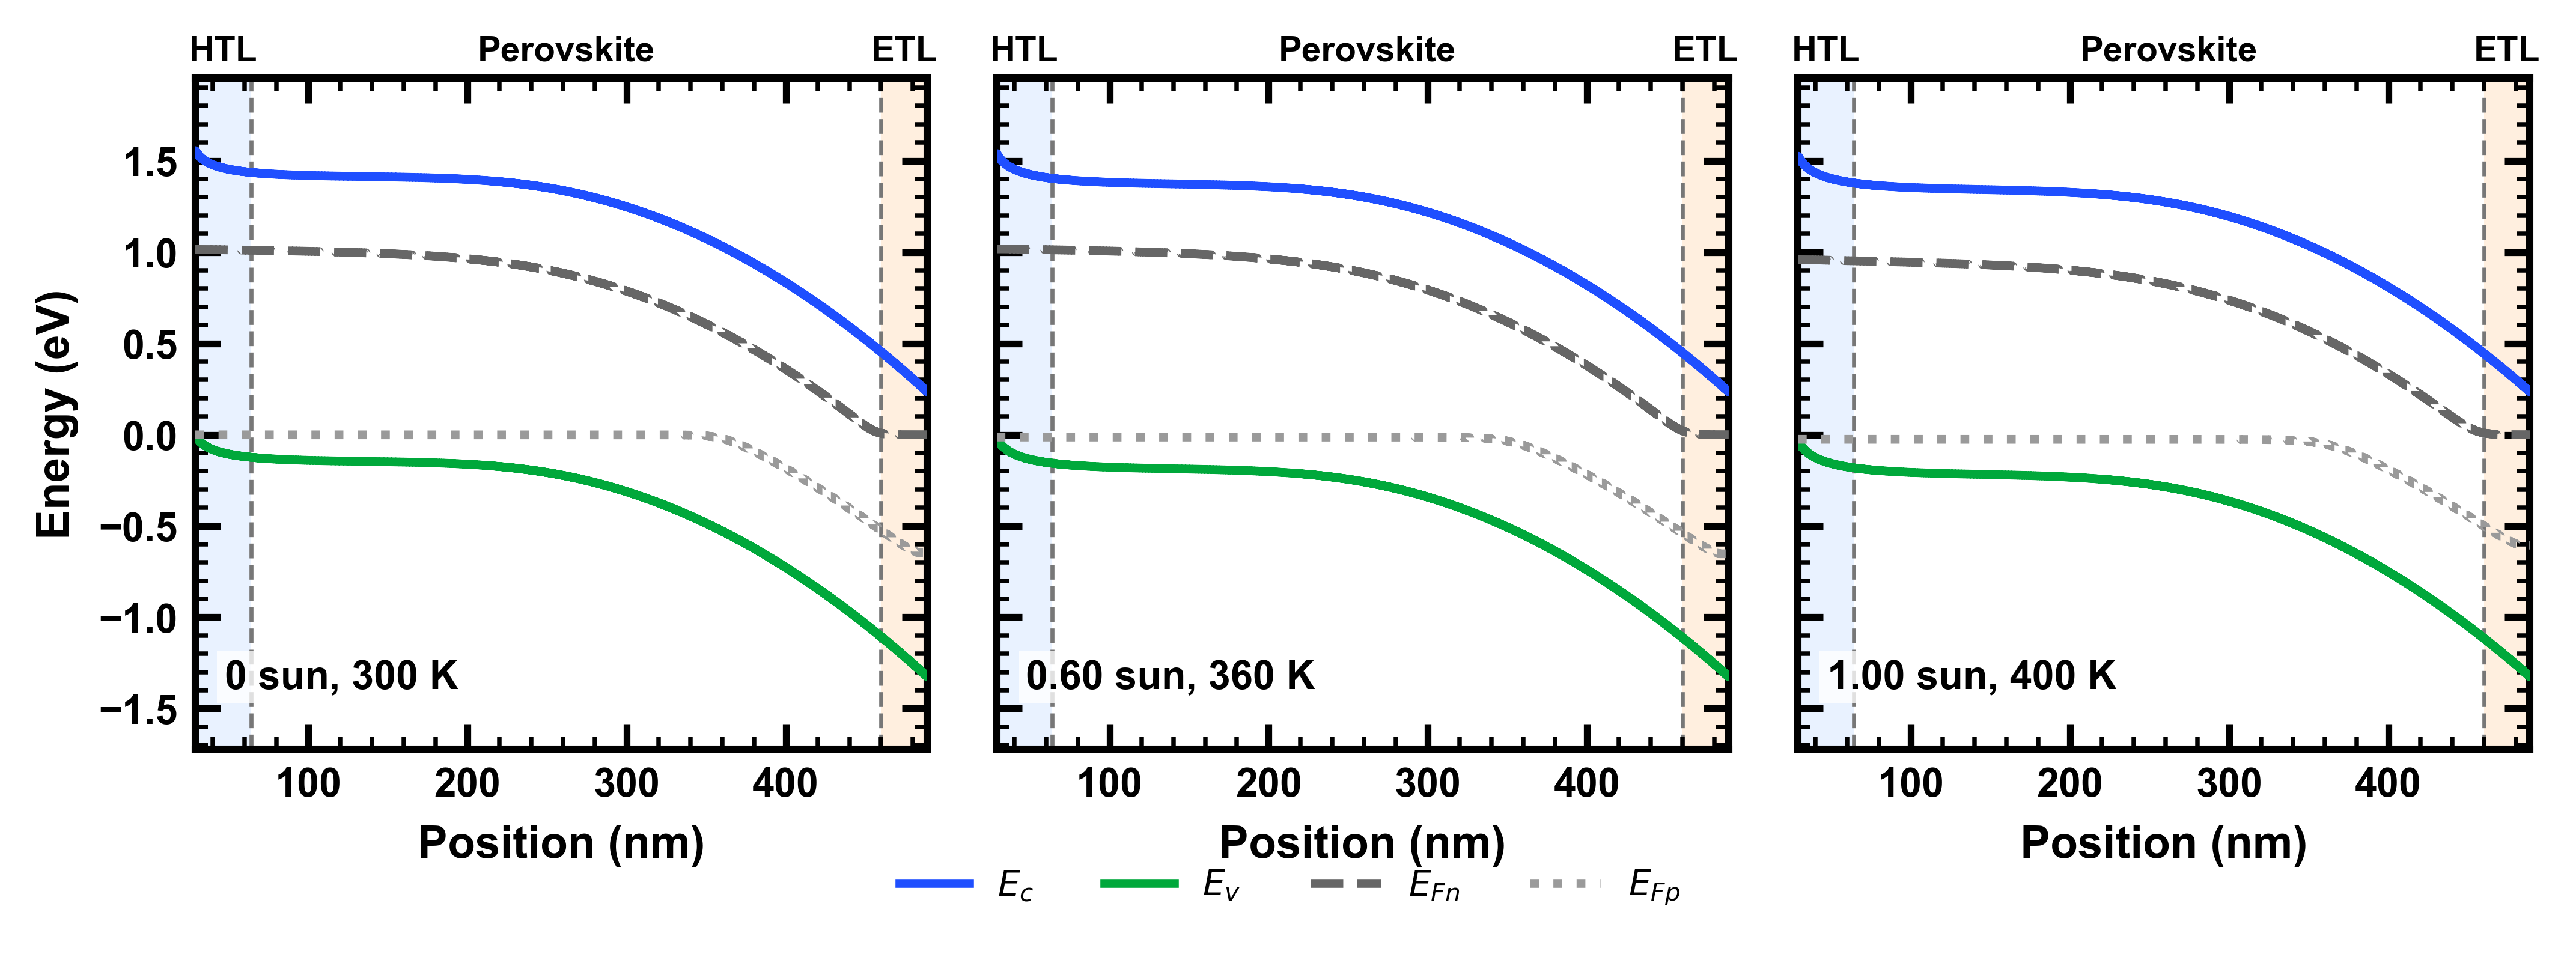
\includegraphics[width=\textwidth]{outputs/figures/comsol_architecture_stress_grid/baseline_pin_band_diagrams_selected_cases.png}
\caption{Selected COMSOL band diagrams from the newest aging-profile exports.
The panels compare final 1000 h profiles for representative low-, medium-, and
high-stress cases. The shaded regions identify the HTL side, perovskite
absorber, and ETL side without reversing the exported coordinate.}
\label{fig:band_diagrams_selected_cases}
\end{figure}

The profile-grid summary in Fig.~\ref{fig:profile_grid_final_state_summary}
establishes that the internal state variables can be exported and summarized
across stress conditions. Figures~\ref{fig:spatial_profiles_selected_cases}
and~\ref{fig:spatial_profiles_high_stress} use those same exports to show the
spatial form of the ion, trap, effective trap-density, and electric-field
states directly. These profiles support the qualitative interpretation that
aging is spatially localized near the transport-layer interfaces, with the
largest trap-density response under combined high light and high temperature.
The perovskite-domain average of $u_{\mathrm{ion}}$ in
Table~\ref{tab:spatial_profile_summary} is included as a normalization
diagnostic; strict ion conservation should be checked with the same COMSOL
integration operator used in the model.

\begin{figure}[H]
\centering
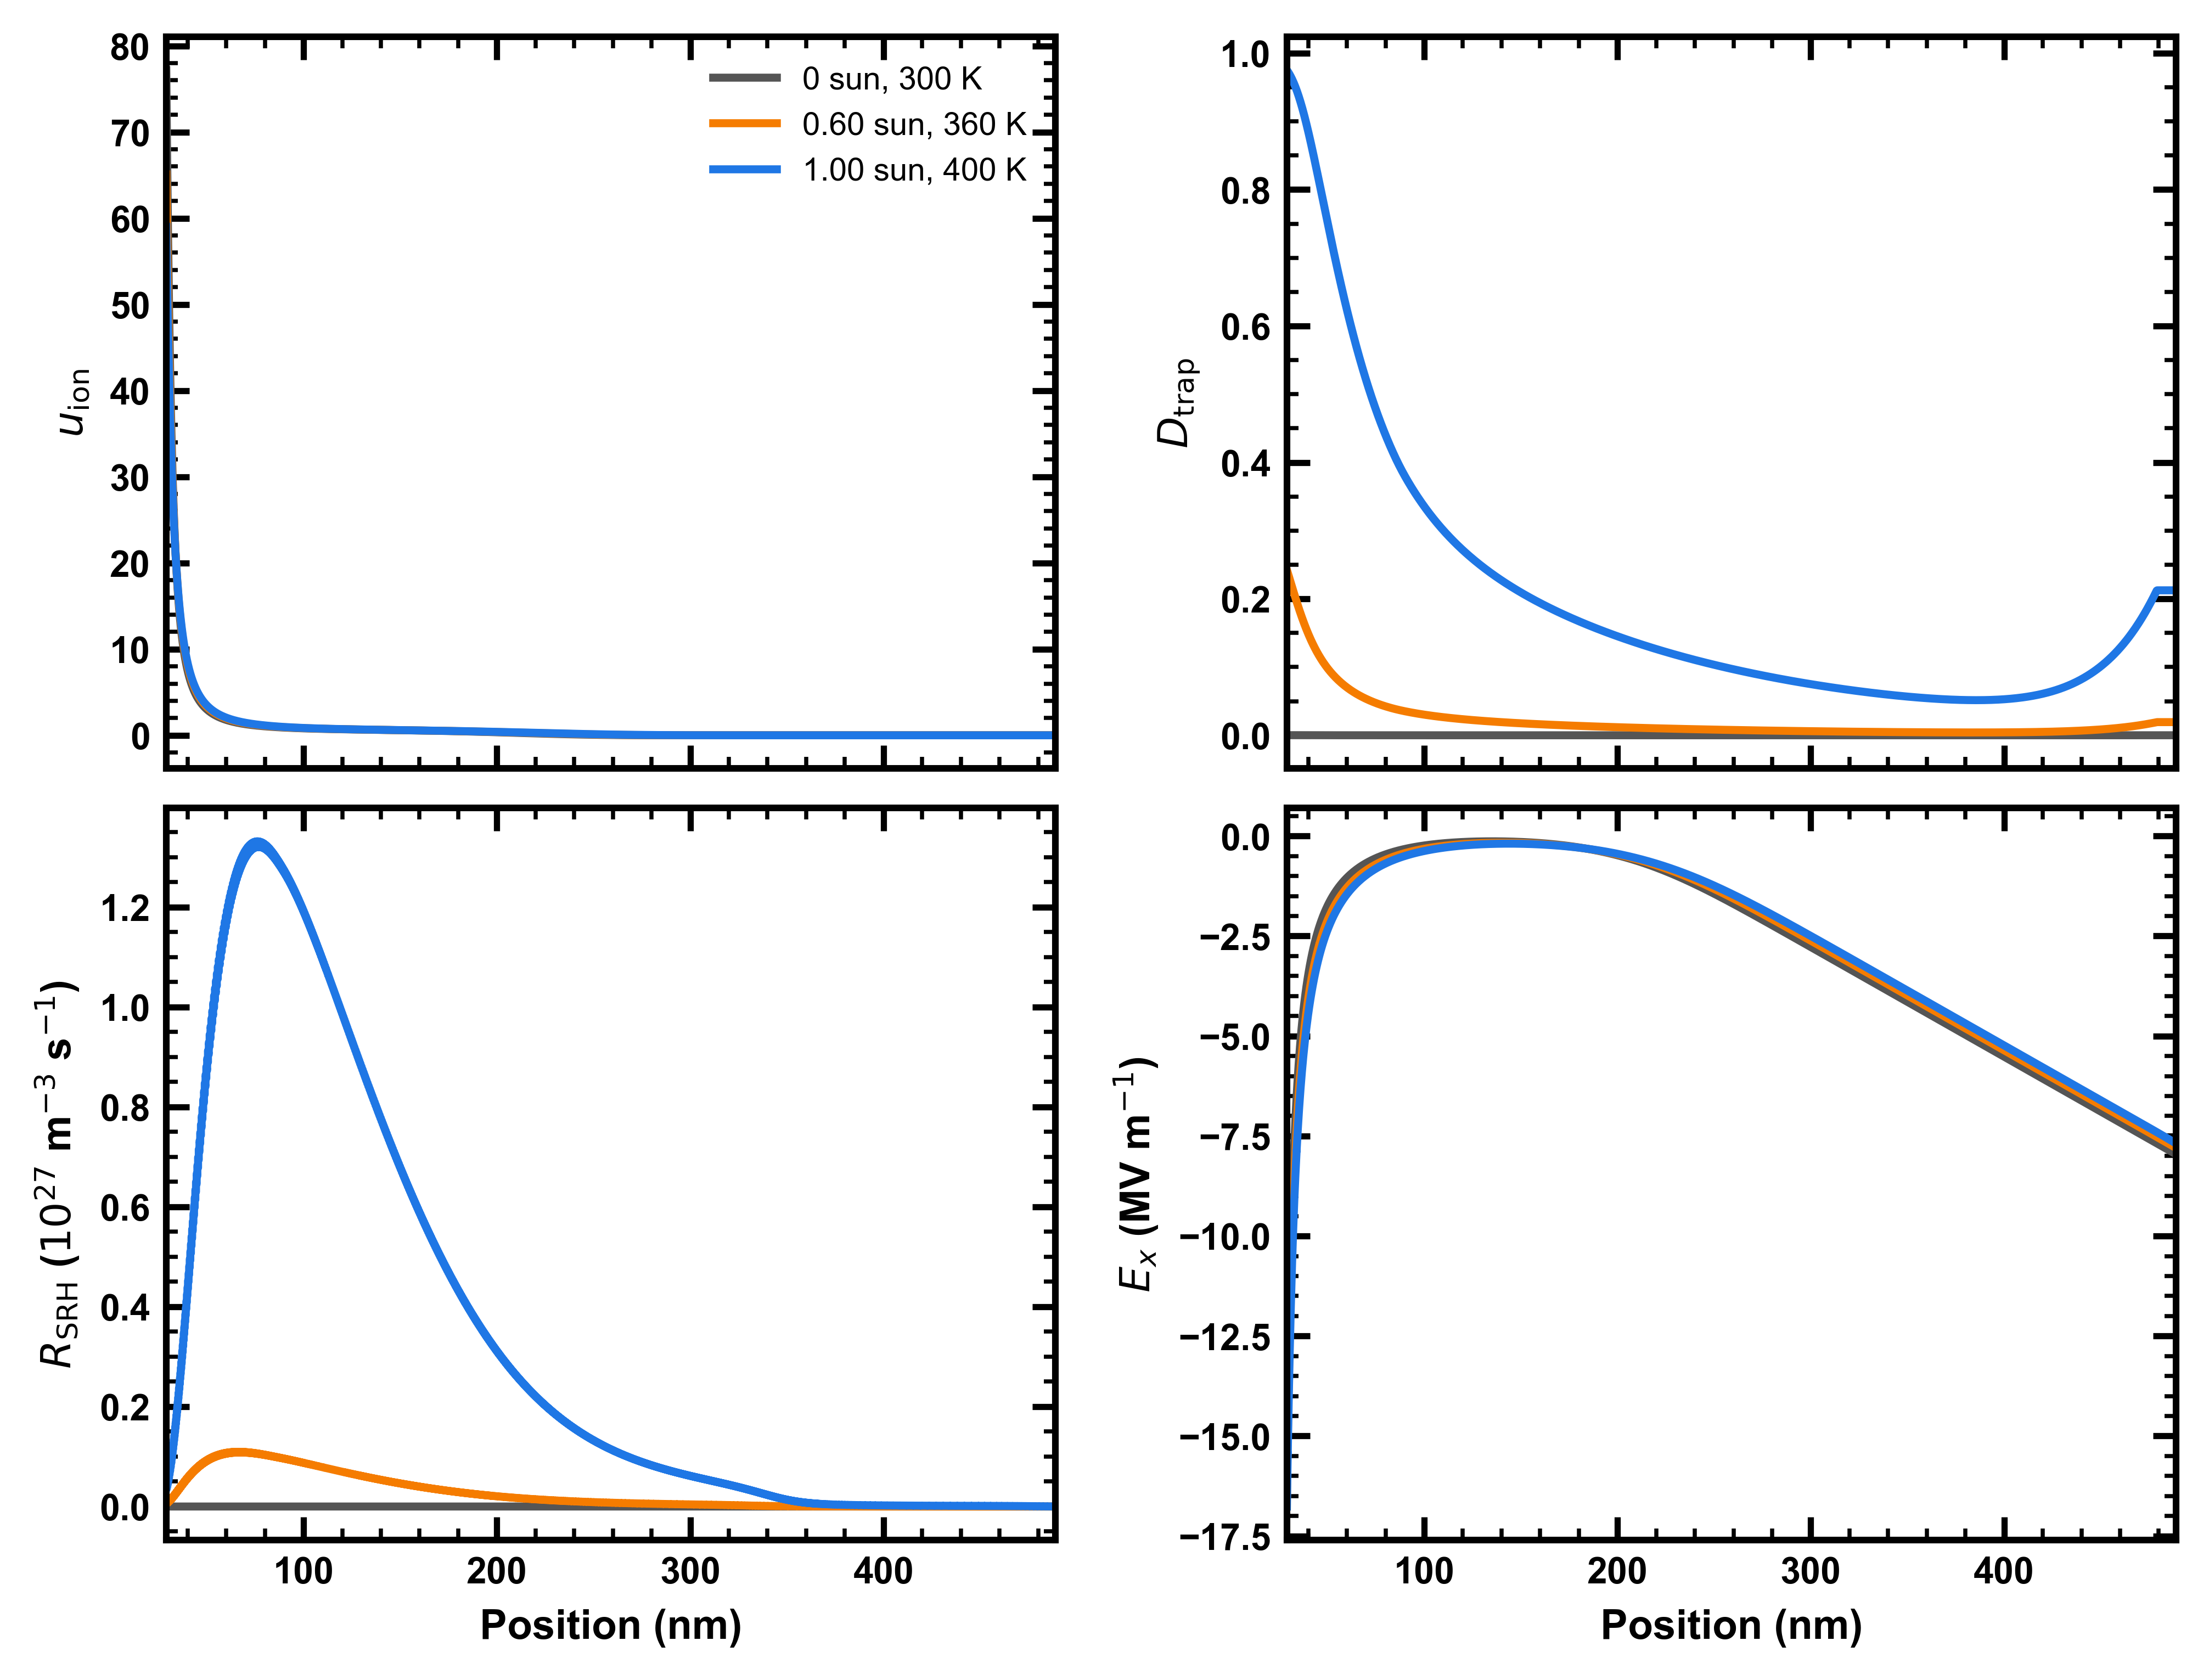
\includegraphics[width=0.92\textwidth]{outputs/figures/comsol_architecture_stress_grid/baseline_pin_spatial_profiles_selected_cases.png}
\caption{Selected final-state spatial profiles from the baseline p-i-n
light-temperature grid. The panels compare low-, medium-, and high-stress
cases at 1000 h equivalent aging for normalized ion concentration, latent trap
damage, effective trap density, and electric field. Shaded regions identify
the HTL and ETL sides without reversing the COMSOL coordinate.}
\label{fig:spatial_profiles_selected_cases}
\end{figure}

\begin{figure}[H]
\centering
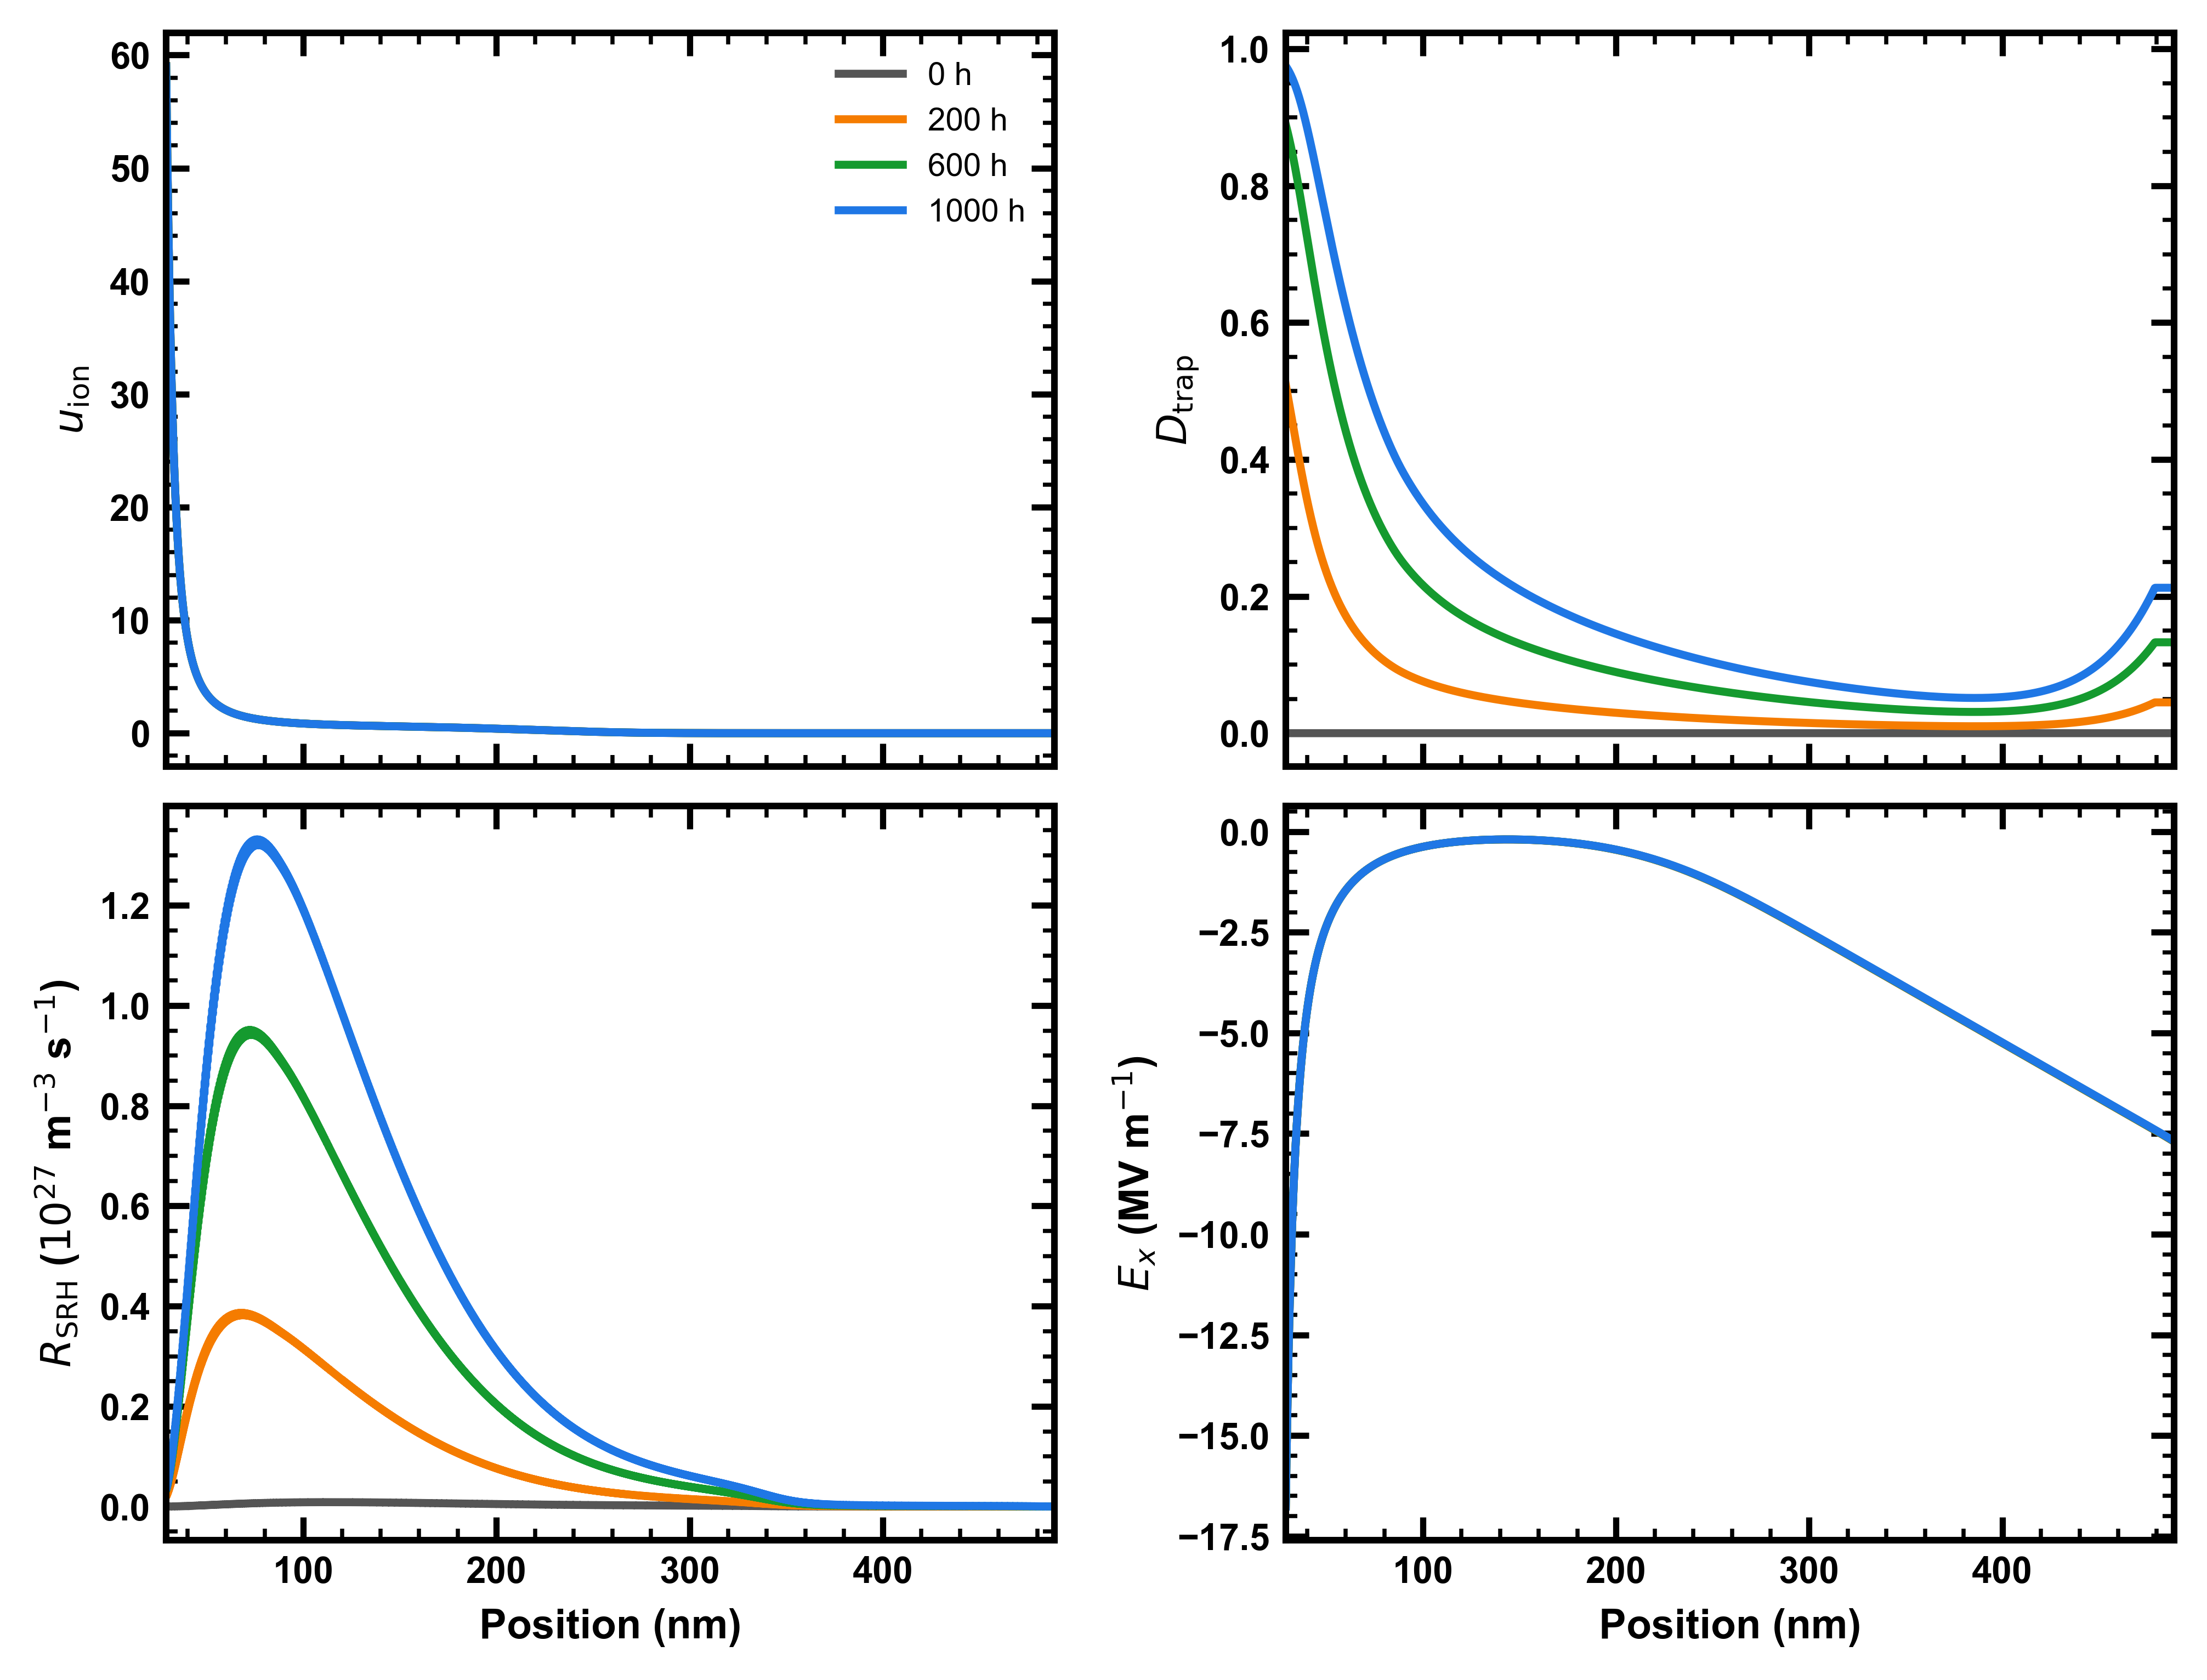
\includegraphics[width=0.92\textwidth]{outputs/figures/comsol_architecture_stress_grid/baseline_pin_spatial_profiles_high_stress_time_evolution.png}
\caption{Time evolution of the high-stress spatial profile at 1 sun and
400 K. The interface-localized increase in $D_{\mathrm{trap}}$ and
$N_{t,\mathrm{eff}}$ shows how the latent damage state maps onto an electronic
recombination parameter while the mobile-ion profile remains strongly
interfacial.}
\label{fig:spatial_profiles_high_stress}
\end{figure}

\begin{table}[H]
\centering
\caption{Selected spatial-profile summaries at 1000 h equivalent aging.}
\label{tab:spatial_profile_summary}
\begin{tabular}{@{}lrrrr@{}}
\toprule
Case & Mean $u_{\mathrm{ion}}$ & Max $u_{\mathrm{ion}}$ & Max $D_{\mathrm{trap}}$ & Mean $N_{t,\mathrm{eff}}$ (cm$^{-3}$) \\
\midrule
0 sun, 300 K & 0.27 & 1.52 & 5.16e-05 & 1.009e+15 \\
0.60 sun, 360 K & 0.287 & 1.65 & 0.0617 & 7.429e+15 \\
1.00 sun, 400 K & 0.298 & 1.72 & 0.574 & 7.488e+16 \\
\bottomrule
\end{tabular}
\end{table}


In Table~\ref{tab:spatial_profile_summary}, the perovskite-domain mean of
$u_{\mathrm{ion}}$ is a sampled-grid normalization diagnostic rather than a
strict conservation integral. Because $u_{\mathrm{ion}}=c_{\mathrm{ion}}/
c_{\mathrm{ion},0}$ is a normalized concentration, the physically relevant
conservation check is the integrated inventory ratio,
\begin{equation}
\frac{\int_{\mathrm{PVK}} c_{\mathrm{ion}}(x,t)\,dx}
{\int_{\mathrm{PVK}} c_{\mathrm{ion}}(x,0)\,dx},
\end{equation}
evaluated with the same COMSOL integration operator and domain selection used
by the model.

The first dedicated COMSOL DIT baseline-control export is shown in
Fig.~\ref{fig:dit_baseline_control}. This dark, no-scan transient has
\texttt{light\_on = 0} and \texttt{use\_scan = 0}. It captures the
electronic/capacitive switching response that must be subtracted from a
mobile-ion-active pulse before integrating ionic charge. The tail current is
near zero after the switching transient, so the export is suitable as a
background-control data product. It does not by itself define a final mobile-ion
concentration because the matched mobile-ion-active pulse must be processed
with the same time base and voltage protocol.

\begin{figure}[H]
\centering
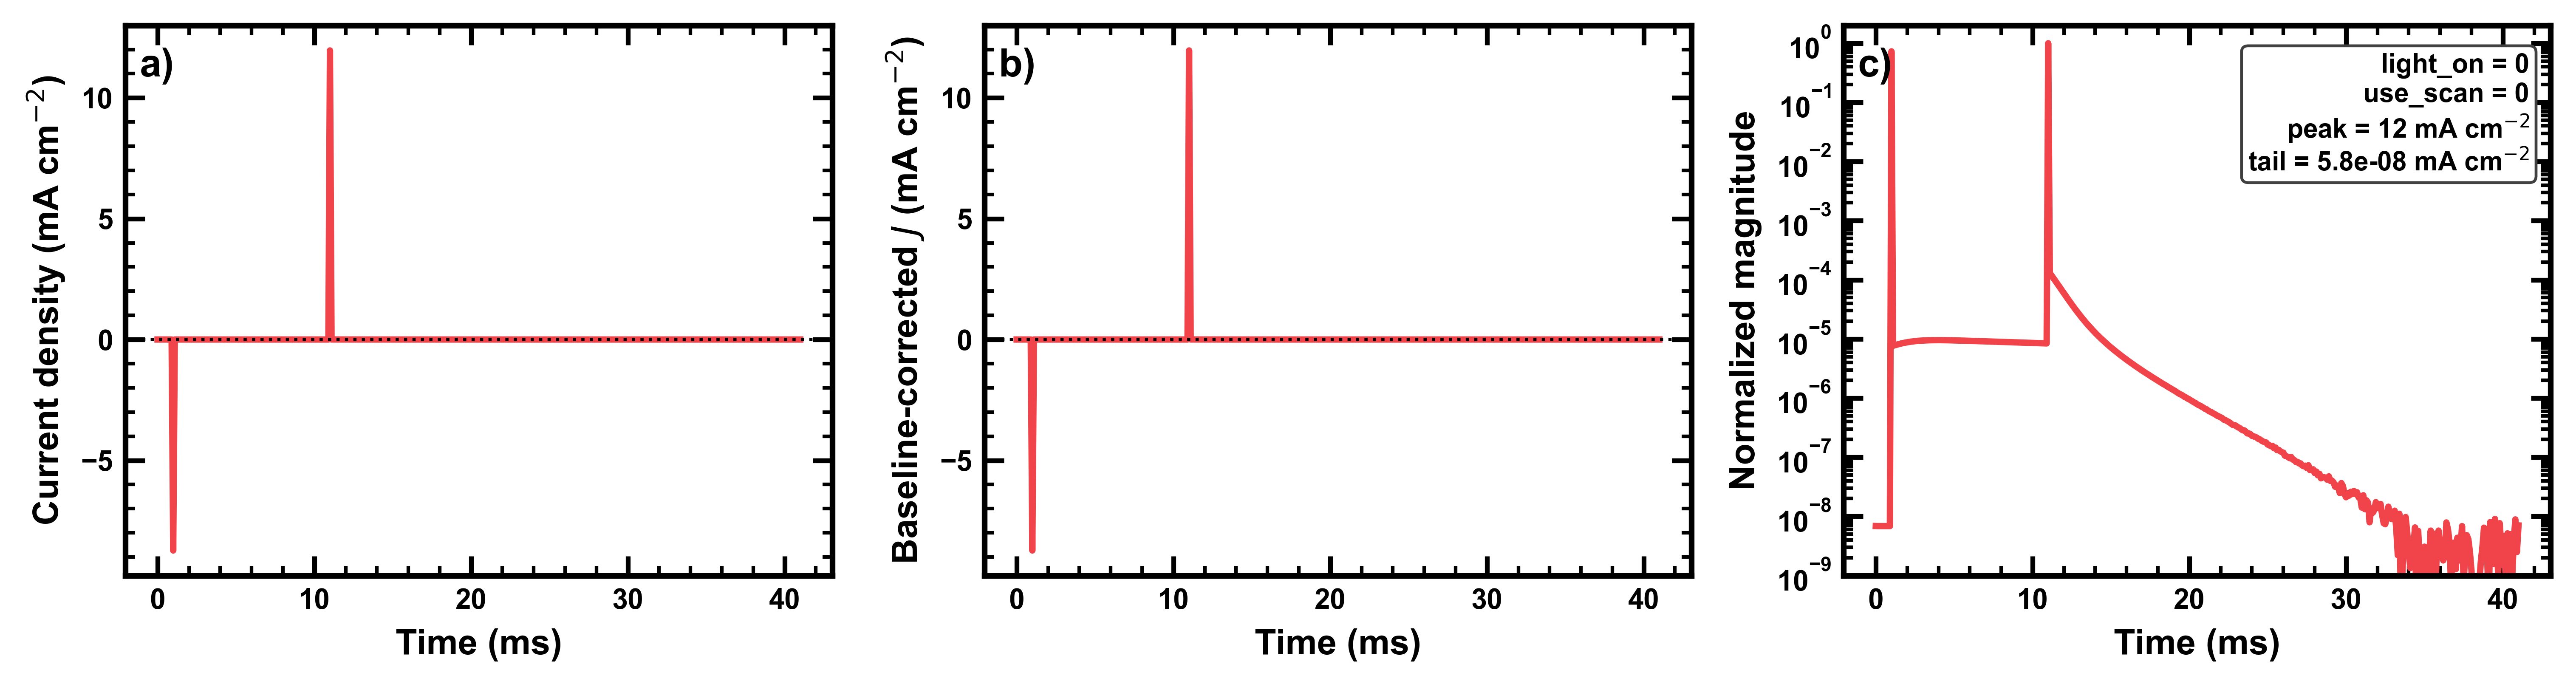
\includegraphics[width=\textwidth]{outputs/figures/dit/dit_baseline_control.png}
\caption{COMSOL DIT baseline-control transient from the dark, no-scan export.
The large switching spikes define the electronic/capacitive background, while
the post-switching tail approaches the numerical current-density floor. This
control is the required background trace for later baseline-corrected ionic
charge integration.}
\label{fig:dit_baseline_control}
\end{figure}

The DIT governing equations and extraction methods are implemented or
documented, but the quantitative ion-density result is not claimed as a final
result until the matched mobile-ion-active current is exported and baseline
subtracted against this control.

\section{Discussion}

The simulation results support the central modeling approach. The COMSOL model
connects electronic drift-diffusion, mobile-ion redistribution, and
degradation-state mappings in a single auditable framework. The strongest
qualitative result is mechanism separation: trap density, shunting, contact
resistance, photogeneration, and ionic charge produce different J--V
signatures. The main limitation is calibration. Stronger claims require matched
baseline J--V data, controlled aging data, ion-sensitive measurements, and
uncertainty estimates for the degradation amplitudes.
